\documentclass{scrartcl}
\usepackage{tikz}
\usetikzlibrary{arrows,automata}

\usepackage{comment}
\begin{document}
\hfuzz=\maxdimen
\tolerance=10000
\hbadness=10000

Wen Liang(\texttt{Wen\_Liang@student.uml.edu}) 01724877
\\
\\
\\
\noindent$\textbf{1.3}$
\\
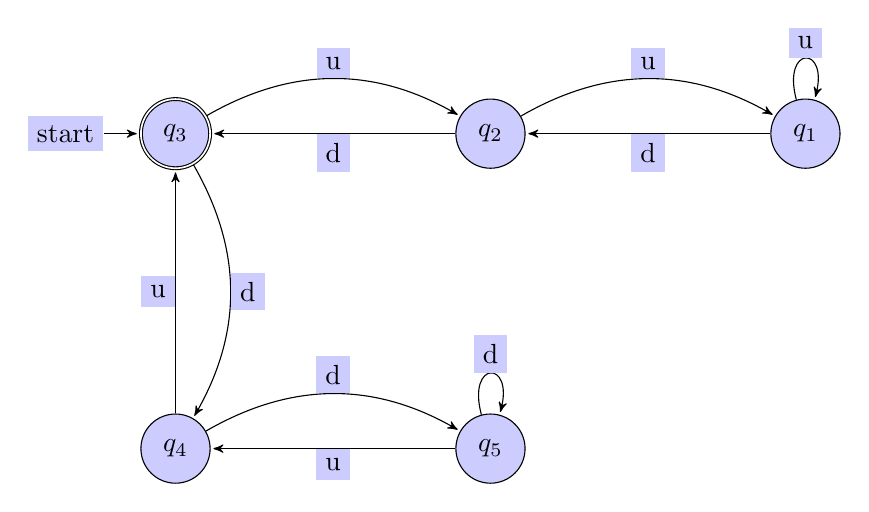
\begin{tikzpicture}[>=stealth',shorten >=1pt,auto,node distance=4cm,every node/.style={fill=blue!20}]
\node[initial,state,accepting	]   (q3)      				{$q_3$};
 \node[state] 	  (q2) [right of=q3]  	{$q_2$};
  \node[state]  	(q1) [right of=q2]  	{$q_1$};
	\node[state]   (q4) [below of=q3]   {$q_4$};
	\node[state]  (q5) [right of=q4]   {$q_5$};
	
	\path[->] (q3)  edge[bend left]	  	node{u} 	(q2)
								edge[bend left]			node{d}		(q4)
								
        (q2) edge  node{d} 		 	(q3)
							edge[bend left] node{u}		(q1)
				(q1) edge [loop above]  node{u}    (q1)
							edge	node{d}		(q2)
				(q4)	edge node{u}	(q3)
							edge[bend left] node{d}	(q5)
				
				(q5)	edge node{u}	(q4)
							edge [loop above] node{d}	(q5);
				
        
\end{tikzpicture}

\noindent$\textbf{1.4}$
\\
\\
\noindent\textbf{a.}
\\
\\
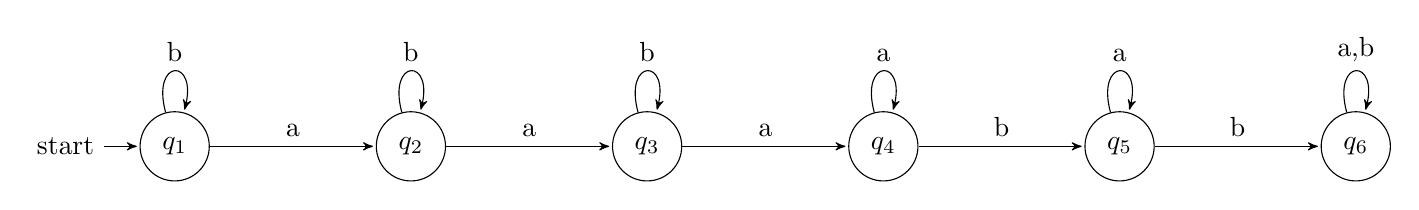
\begin{tikzpicture}[>=stealth',shorten >=1pt,auto,node distance=3cm]

\node[initial,state	]   (q1)      				{$q_1$};
 \node[state] 	  (q2) [right of=q1]  	{$q_2$};
	\node[state]   (q3) [right of=q2]      				{$q_3$};
	\node[state] 	  (q4) [right of=q3]  	{$q_4$};
	\node[state] 	  (q5) [right of=q4]  	{$q_5$};
	\node[state] 	  (q6) [right of=q5]  	{$q_6$};
	
	\path[->] (q1)  edge	  	node{a} 	(q2)
									edge[loop above]	  	node{b} 	(q1)			
        (q2) edge[loop above]  node{b} 		 	(q2)
							edge node{a}		(q3)
					(q3) edge[loop above]  node{b} 		 	(q3)
							edge  node{a} 		 	(q4)
					(q4) edge[loop above]  node{a} 		 	(q4)
							edge  node{b} 		 	(q5)
					(q5) edge[loop above]  node{a} 		 	(q5)
							edge  node{b} 		 	(q6)
					(q6) edge[loop above]  node{a,b} 		 	(q6);
\end{tikzpicture}	


\noindent\textbf{c.}
\\
\\
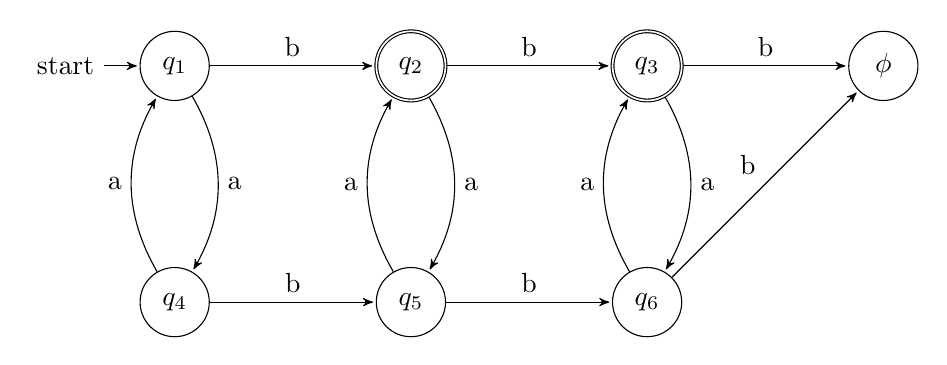
\begin{tikzpicture}[>=stealth',shorten >=1pt,auto,node distance=3cm]

\node[initial,state	]   (q1)      				{$q_1$};
 \node[state,accepting] 	  (q2) [right of=q1]  	{$q_2$};
	\node[state,accepting]   (q3) [right of=q2]      				{$q_3$};
	\node[state] 	  (q4) [below of=q1]  	{$q_4$};
	\node[state] 	  (q5) [below of=q2]  	{$q_5$};
	\node[state] 	  (q6) [below of=q3]  	{$q_6$};
	\node[state] 	  (phi) [right of=q3]  	{$\phi$};
	
	\path[->] (q1)  edge	  	node{b} 	(q2)
									edge[bend left]	  	node{a} 	(q4)			
        (q2) edge node{b} 		 	(q3)
							edge[bend left] node{a}		(q5)
					(q3) edge  node{b} 		 	(phi)
							edge[bend left]  node{a} 		 	(q6)
					(q4) edge[bend left]  node{a} 		 	(q1)
							edge  node{b} 		 	(q5)
					(q5) edge[bend left]  node{a} 		 	(q2)
							edge  node{b} 		 	(q6)
					(q6) edge[bend left]  node{a} 		 	(q3)
								edge  node{b} 		 	(phi);
\end{tikzpicture}	

\noindent\textbf{e.}
\\
\\
\\
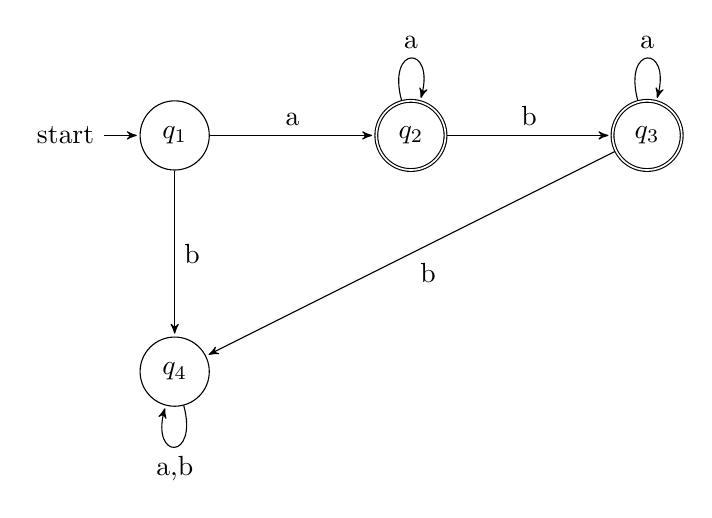
\begin{tikzpicture}[>=stealth',shorten >=1pt,auto,node distance=3cm]

\node[initial,state	]   (q1)      				{$q_1$};
 \node[state,accepting] 	  (q2) [right of=q1]  	{$q_2$};
	\node[state,accepting]   (q3) [right of=q2]      				{$q_3$};
	\node[state] 	  (q4) [below of=q1]  	{$q_4$};
	
	
	\path[->] (q1)  edge	  	node{a} 	(q2)
									edge  	node{b} 	(q4)			
        (q2) edge[loop above]  node{a} 		 	(q2)
							edge node{b}		(q3)
					(q3) edge[loop above]  node{a} 		 	(q3)
							edge  node{b} 		 	(q4)
					(q4) edge[loop below]  node{a,b} 		 	(q4);
							
				
\end{tikzpicture}

\noindent\textbf{f.}
\\
\\
\\
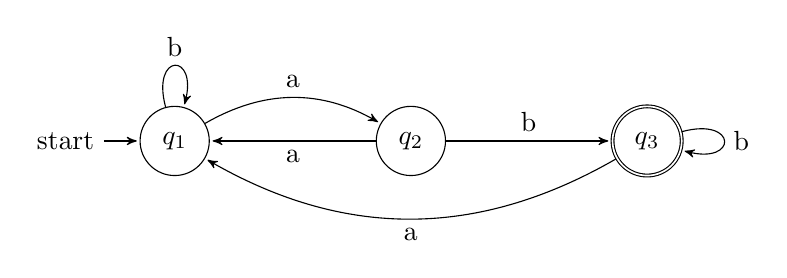
\begin{tikzpicture}[>=stealth',shorten >=1pt,auto,node distance=3cm]

\node[initial,state	]   (q1)      				{$q_1$};
 \node[state] 	  (q2) [right of=q1]  	{$q_2$};
	\node[state,accepting]   (q3) [right of=q2]      				{$q_3$};
	
	
	
	\path[->] (q1)  edge[loop above]	  	node{b} 	(q1)
									edge[bend left]  	node{a} 	(q2)			
        (q2) edge  node{a} 		 	(q1)
							edge node{b}		(q3)
					(q3) edge[loop right]  node{b} 		 	(q3)
							edge[bend left]  node{a}		 	(q1);
				
							
				
\end{tikzpicture}

\noindent\textbf{g.}
\\
\\
\\
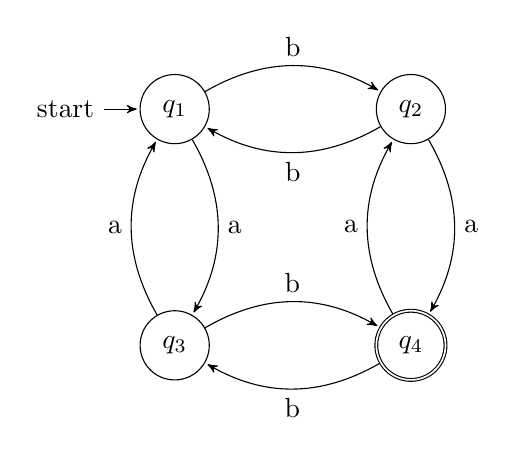
\begin{tikzpicture}[>=stealth',shorten >=1pt,auto,node distance=3cm]

\node[initial,state	]   (q1)      				{$q_1$};
 \node[state] 	  (q2) [right of=q1]  	{$q_2$};
	\node[state]   (q3) [below of=q1]      				{$q_3$};
		\node[state,accepting]   (q4) [below of=q2]      				{$q_4$};
	
	
	\path[->] (q1)  edge[bend left]	  	node{b} 	(q2)
									edge[bend left]  	node{a} 	(q3)			
        (q2) edge[bend left]  node{a} 		 	(q4)
							edge[bend left] node{b}		(q1)
					(q3) edge[bend left]  node{a} 		 	(q1)
							edge[bend left]  node{b}		 	(q4)
						(q4) edge[bend left]  node{a} 		 	(q2)
							edge[bend left]  node{b}		 	(q3);
							
				
\end{tikzpicture}

\noindent$\textbf{1.5}$
\\
\\
\noindent\textbf{c.}
\\
\\
\\
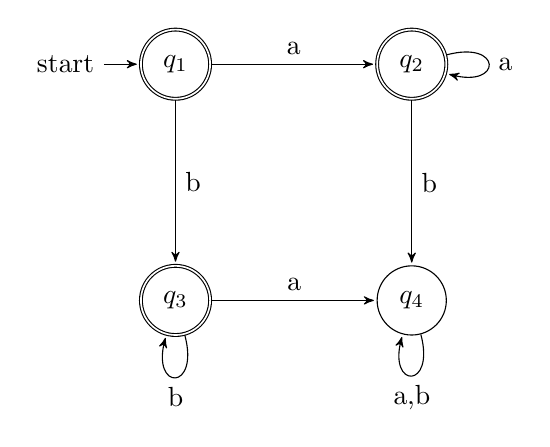
\begin{tikzpicture}[>=stealth',shorten >=1pt,auto,node distance=3cm]

\node[initial,state,accepting]   (q1)      				{$q_1$};
 \node[state,accepting] 	  (q2) [right of=q1]  	{$q_2$};
	\node[state,accepting]   (q3) [below of=q1]      				{$q_3$};
\node[state]   (q4) [below of=q2]      				{$q_4$};

	\path[->] (q1)  edge	  	node{a} 	(q2)
									edge	  	node{b} 	(q3)					
        (q2) edge[loop right] node{a} 		 	(q2)
						edge node{b} 		 	(q4)
							
					(q3) edge[loop below]  node{b} 		 	(q3)
								edge  node{a} 		 	(q4)
						(q4) edge[loop below]  node{a,b} 		 	(q4);
							
					
					
	\end{tikzpicture}

\noindent\textbf{d.}
\\
\\
\\
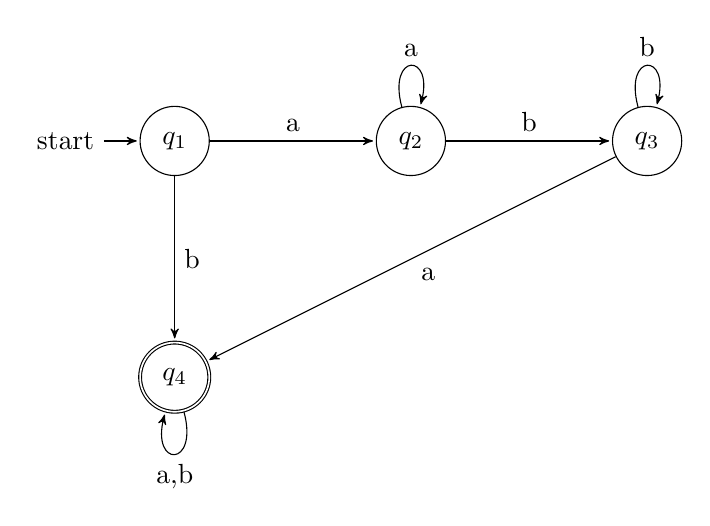
\begin{tikzpicture}[>=stealth',shorten >=1pt,auto,node distance=3cm]

\node[initial,state]   (q1)      				{$q_1$};
 \node[state] 	  (q2) [right of=q1]  	{$q_2$};
	\node[state]   (q3) [right of=q2]      				{$q_3$};
\node[state,accepting]   (q4) [below of=q1]      				{$q_4$};

	\path[->] (q1)  edge	  	node{a} 	(q2)
									edge	  	node{b} 	(q4)					
        (q2) edge[loop above] node{a} 		 	(q2)
						edge node{b} 		 	(q3)
							
					(q3) edge[loop above]  node{b} 		 	(q3)
								edge  node{a} 		 	(q4)
						(q4) edge[loop below]  node{a,b} 		 	(q4);
							
					
					
	\end{tikzpicture}
	
\noindent\textbf{e.}
\\
\\
\\
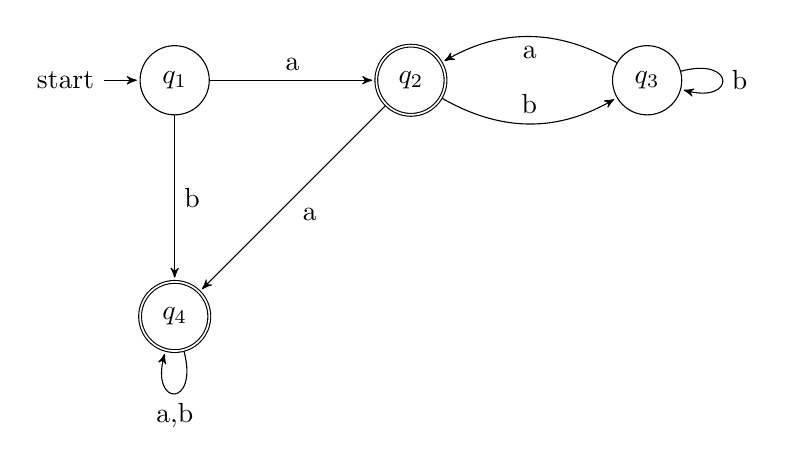
\begin{tikzpicture}[>=stealth',shorten >=1pt,auto,node distance=3cm]

\node[initial,state]   (q1)      				{$q_1$};
 \node[state,accepting] 	  (q2) [right of=q1]  	{$q_2$};
\node[state]   (q3) [right of=q2]      				{$q_3$};
\node[state,accepting]   (q4) [below of=q1]      				{$q_4$};

	\path[->] (q1)  edge	  	node{a} 	(q2)
									edge	  	node{b} 	(q4)					
        (q2) edge node{a} 		 	(q4)
						edge[bend right] node{b} 		 	(q3)
							
					(q3) edge[loop right]  node{b} 		 	(q3)
								edge[bend right]  node{a} 		 	(q2)
						(q4) edge[loop below]  node{a,b} 		 	(q4);
							
					
					
	\end{tikzpicture}
\\
\\

\noindent\textbf{f.}
\\
\\
\\
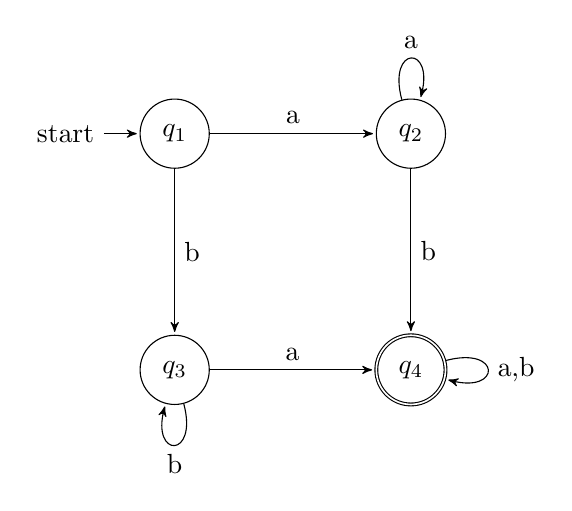
\begin{tikzpicture}[>=stealth',shorten >=1pt,auto,node distance=3cm]

\node[initial,state]   (q1)      				{$q_1$};
 \node[state] 	  (q2) [right of=q1]  	{$q_2$};
	\node[state]   (q3) [below of=q1]      				{$q_3$};
\node[state,accepting]   (q4) [below of=q2]      				{$q_4$};

	\path[->] (q1)  edge	  	node{a} 	(q2)
									edge	  	node{b} 	(q3)					
        (q2) edge[loop above] node{a} 		 	(q2)
						edge node{b} 		 	(q4)
							
					(q3) edge[loop below]  node{b} 		 	(q3)
								edge  node{a} 		 	(q4)
						(q4) edge[loop right]  node{a,b} 		 	(q4);
							
					
					
	\end{tikzpicture}
		
\noindent\textbf{g.}
\\
\\
\\
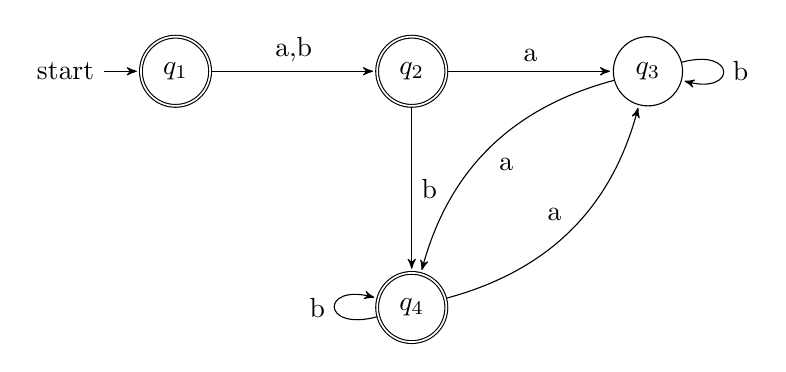
\begin{tikzpicture}[>=stealth',shorten >=1pt,auto,node distance=3cm]

\node[initial,state,accepting]   (q1)      				{$q_1$};
 \node[state,accepting] 	  (q2) [right of=q1]  	{$q_2$};
	\node[state]   (q3) [right of=q2]      				{$q_3$};
\node[state,accepting]   (q4) [below of=q2]      				{$q_4$};

	\path[->] (q1)  edge	  	node{a,b} 	(q2)
														
        (q2) edge node{a} 		 	(q3)
						edge node{b} 		 	(q4)
							
					(q3) edge[bend right]  node{a} 		 	(q4)
								edge[loop right]  node{b} 		 	(q3)
						(q4) edge[bend right]  node{a} 		 	(q3)
								edge[loop left]  node{b} 		 	(q4);	
					
					
		\end{tikzpicture}	
		
\noindent\textbf{h.}
\\
\\
\\
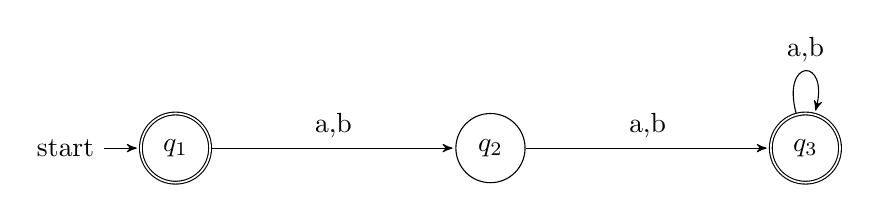
\begin{tikzpicture}[>=stealth',shorten >=1pt,auto,node distance=4cm]

\node[initial,state,accepting]   (q1)      				{$q_1$};
 \node[state] 	  (q2) [right of=q1]  	{$q_2$};
	\node[state,accepting	]   (q3) [right of=q2]      				{$q_3$};


	\path[->] (q1)  edge	  	node{a,b} 	(q2)
														
        (q2) edge node{a,b} 		 	(q3)
							
					(q3) edge[loop above]  node{a,b} 		 	(q3);
						
					
		\end{tikzpicture}	






\noindent$\textbf{1.6}$
\\
\\
\\
\noindent\textbf{a.}
\\
\\
\\
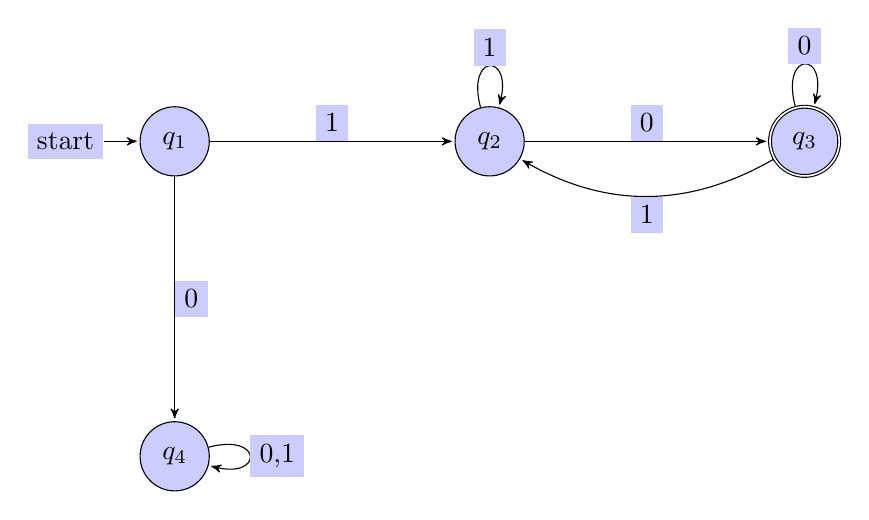
\begin{tikzpicture}[>=stealth',shorten >=1pt,auto,node distance=4cm,every node/.style={fill=blue!20}]

\node[initial,state	]   (q1)      				{$q_1$};
 \node[state] 	  (q2) [right of=q1]  	{$q_2$};
	\node[state,accepting	]   (q3) [right of=q2]      				{$q_3$};
	\node[state] 	  (q4) [below of=q1]  	{$q_4$};

	\path[->] (q1)  edge	  	node{1} 	(q2)
									edge	  	node{0} 	(q4)
								
        (q2) edge[loop above]  node{1} 		 	(q2)
							edge node{0}		(q3)
					(q3) edge[loop above]  node{0} 		 	(q3)
							edge[bend left]  node{1} 		 	(q2)
					(q4) edge[loop right]  node{0,1} 		 	(q4);		
							
					
		\end{tikzpicture}	
		
\noindent\textbf{b.}
\\
\\
\\
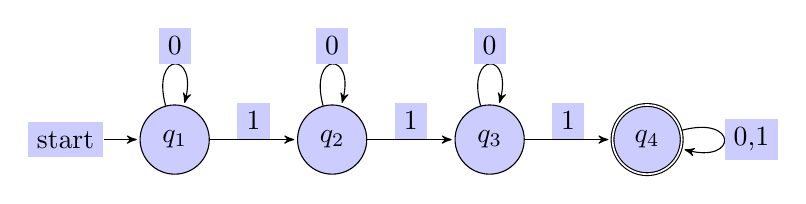
\begin{tikzpicture}[>=stealth',shorten >=1pt,auto,node distance=2cm,every node/.style={fill=blue!20}]

\node[initial,state	]   (q1)      				{$q_1$};
 \node[state] 	  (q2) [right of=q1]  	{$q_2$};
	\node[state	]   (q3) [right of=q2]      				{$q_3$};
	\node[state,accepting] 	  (q4) [right of=q3]  	{$q_4$};

	\path[->] (q1)  edge	  	node{1} 	(q2)
									edge[loop above]	  	node{0} 	(q1)
								
        (q2) edge[loop above]  node{0} 		 	(q2)
							edge node{1}		(q3)
					(q3) edge[loop above]  node{0} 		 	(q3)
							edge  node{1} 		 	(q4)
					(q4) edge[loop right]  node{0,1} 		 	(q4);		
							
					
		\end{tikzpicture}	
		
\noindent\textbf{c.}
\\
\\ 
\\
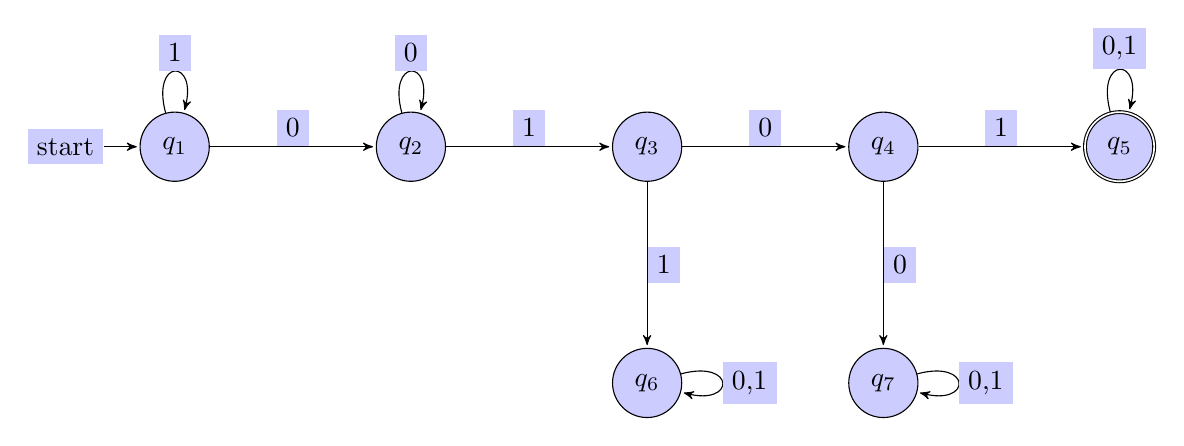
\begin{tikzpicture}[>=stealth',shorten >=1pt,auto,node distance=3cm,every node/.style={fill=blue!20}]

\node[initial,state	]   (q1)      				{$q_1$};
 \node[state] 	  (q2) [right of=q1]  	{$q_2$};
	\node[state	]   (q3) [right of=q2]      				{$q_3$};
	\node[state] 	  (q4) [right of=q3]  	{$q_4$};
	\node[state,accepting] 	  (q5) [right of=q4]  	{$q_5$};
		\node[state] 	  (q6) [below of=q3]  	{$q_6$};
			\node[state] 	  (q7) [below of=q4]  	{$q_7$};

	\path[->] (q1)  edge	  	node{0} 	(q2)
									edge[loop above]	  	node{1} 	(q1)
								
        (q2) edge[loop above]  node{0} 		 	(q2)
							edge node{1}		(q3)
					(q3) edge  node{1} 		 	(q6)
							edge  node{0} 		 	(q4)
					(q4) edge  node{0} 		 	(q7)
								edge  node{1} 		 	(q5)
						(q5) edge[loop above]  node{0,1} 		 	(q5)
						(q6) edge[loop right]  node{0,1} 		 	(q6)
						(q7) edge[loop right]  node{0,1} 		 	(q7);
						
							
					
		\end{tikzpicture}	

\noindent\textbf{d.}
\\
\\
\\
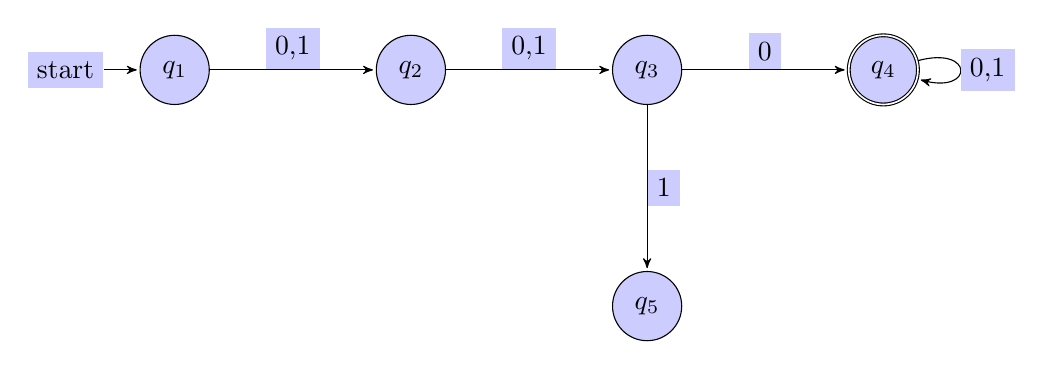
\begin{tikzpicture}[>=stealth',shorten >=1pt,auto,node distance=3cm,every node/.style={fill=blue!20}]

\node[initial,state	]   (q1)      				{$q_1$};
 \node[state] 	  (q2) [right of=q1]  	{$q_2$};
	\node[state	]   (q3) [right of=q2]      				{$q_3$};
	\node[state,accepting] 	  (q4) [right of=q3]  	{$q_4$};
	\node[state	]   (q5) [below of=q3]      				{$q_5$};
	
	\path[->] (q1)  edge	  	node{0,1} 	(q2)
															
        (q2) edge  node{0,1} 		 	(q3)
						
					(q3) edge  node{0} 		 	(q4)
							edge  node{1} 		 	(q5)
							
					(q4) edge[loop right]  node{0,1} 		 	(q4);
								
		\end{tikzpicture}	
	
\noindent\textbf{e.}
\\
\\
\\
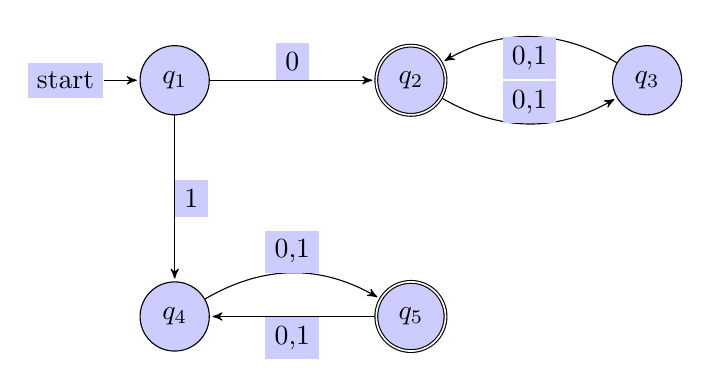
\begin{tikzpicture}[>=stealth',shorten >=1pt,auto,node distance=3cm,every node/.style={fill=blue!20}]

\node[initial,state	]   (q1)      				{$q_1$};
 \node[state,accepting] 	  (q2) [right of=q1]  	{$q_2$};
	\node[state	]   (q3) [right of=q2]      				{$q_3$};
	\node[state] 	  (q4) [below of=q1]  	{$q_4$};
	\node[state,accepting]   (q5) [right of=q4]      				{$q_5$};
	
	\path[->] (q1)  edge	  	node{0} 	(q2)
										edge	  	node{1} 	(q4)				
        (q2) edge[bend right]  node{0,1} 		 	(q3)
						
					(q3) edge[bend right]  node{0,1} 		 	(q2)
						
							
					(q4) edge[bend left]  node{0,1} 		 	(q5)
					(q5) edge  node{0,1} 		 	(q4);
								
		\end{tikzpicture}	


\noindent\textbf{f.}
\\
\\
\\
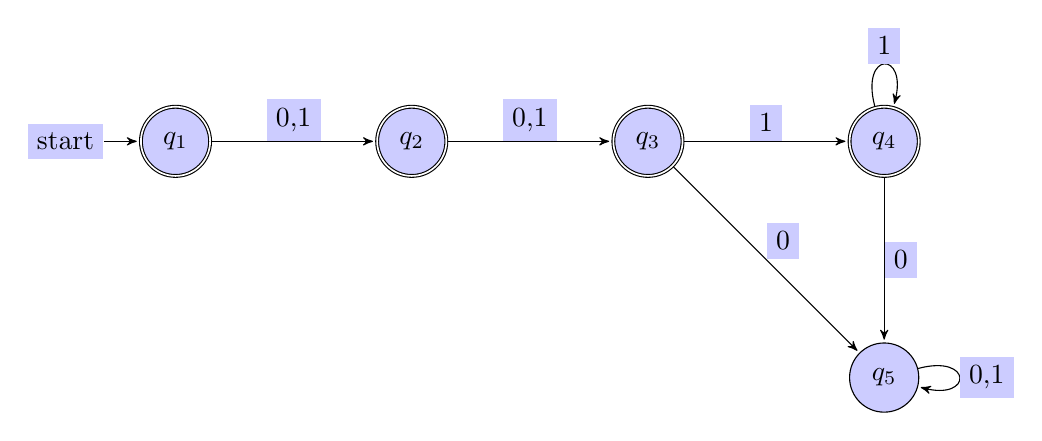
\begin{tikzpicture}[>=stealth',shorten >=1pt,auto,node distance=3cm,every node/.style={fill=blue!20}]

\node[initial,state,accepting	]   (q1)      				{$q_1$};
 \node[state,accepting] 	  (q2) [right of=q1]  	{$q_2$};
	\node[state,accepting	]   (q3) [right of=q2]      				{$q_3$};
	\node[state,accepting] 	  (q4) [right of=q3]  	{$q_4$};
	\node[state]   (q5) [below of=q4]      				{$q_5$};
	
	\path[->] (q1)  edge	  	node{0,1} 	(q2)
							
        (q2) edge  node{0,1} 		 	(q3)
						
					(q3) edge  node{1} 		 	(q4)
							edge  node{0} 		 	(q5)	
							
					(q4) edge[loop above]  node{1} 		 	(q4)
								edge     node{0} 		 	(q5)
					(q5) edge[loop right]  node{0,1} 		 	(q5);
								
	\end{tikzpicture}
	
\noindent\textbf{g.}
\\
\\
\\
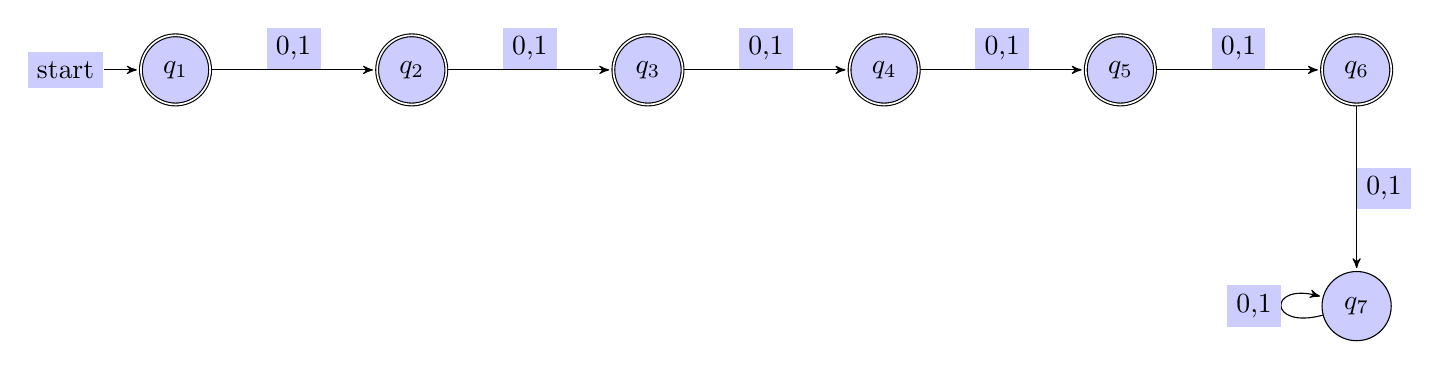
\begin{tikzpicture}[>=stealth',shorten >=1pt,auto,node distance=3cm,every node/.style={fill=blue!20}]

\node[initial,state,accepting	]   (q1)      				{$q_1$};
 \node[state,accepting] 	  (q2) [right of=q1]  	{$q_2$};
	\node[state,accepting	]   (q3) [right of=q2]      				{$q_3$};
	\node[state,accepting] 	  (q4) [right of=q3]  	{$q_4$};
	\node[state,accepting]   (q5) [right of=q4]      				{$q_5$};
	\node[state,accepting]   (q6) [right of=q5]      				{$q_6$};
		\node[state]   (q7) [below of=q6]      				{$q_7$};
	
	\path[->] (q1)  edge	  	node{0,1} 	(q2)
							
        (q2) edge  node{0,1} 		 	(q3)
						
					(q3) edge  node{0,1} 		 	(q4)
														
					(q4) edge  node{0,1} 		 	(q5)
						
					(q5) edge  node{0,1} 		 	(q6)
					
					(q6) edge  node{0,1} 		 	(q7)
					
					(q7) edge[loop left]  node{0,1} 		 	(q7);
				

								
	\end{tikzpicture}
	
\noindent\textbf{h.}
\\
\\
\\
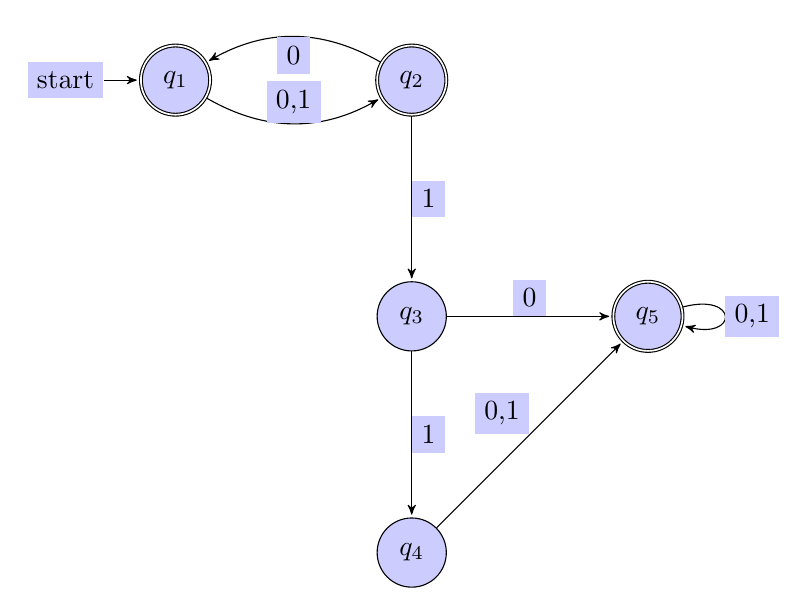
\begin{tikzpicture}[>=stealth',shorten >=1pt,auto,node distance=3cm,every node/.style={fill=blue!20}]

\node[initial,state,accepting	]   (q1)      				{$q_1$};
 \node[state,accepting] 	  (q2) [right of=q1]  	{$q_2$};
	\node[state]   (q3) [below of=q2]      				{$q_3$};
	\node[state] 	  (q4) [below of=q3]  	{$q_4$};
	\node[state,accepting]   (q5) [right of=q3]      				{$q_5$};
	
	\path[->] (q1)  edge[bend right]	  	node{0,1} 	(q2)
							
        (q2) edge[bend right]  node{0} 		 	(q1)
							edge  node{1} 		 	(q3)
						
					(q3) edge  node{0} 		 	(q5)
								edge  node{1} 		 	(q4)
														
					(q4) edge  node{0,1} 		 	(q5)
						
					(q5) edge[loop right]  node{0,1} 		 	(q5);
					
						
	\end{tikzpicture}
	
	\noindent\textbf{i.}
	\\
	\\
	\\
	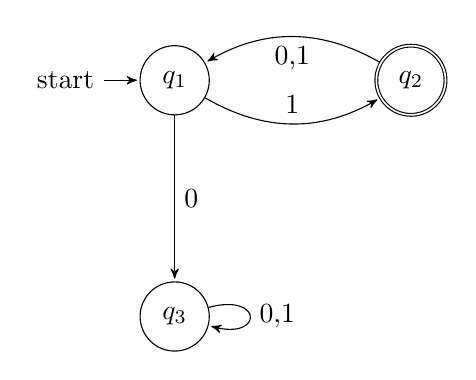
\begin{tikzpicture}[>=stealth',shorten >=1pt,auto,node distance=3cm]

\node[initial,state	]   (q1)      				{$q_1$};
 \node[state,accepting] 	  (q2) [right of=q1]  	{$q_2$};
	\node[state]   (q3) [below of=q1]      				{$q_3$};
	
	
	\path[->] (q1)  edge[bend right]	  	node{1} 	(q2)
							
									edge  node{0} 		 	(q3)
	
					(q2) edge[bend right]  node{0,1} 		 	(q1)
							
														
					(q3) edge[loop right]  node{0,1} 		 	(q3);
					
					
						
	\end{tikzpicture}
	
	\noindent\textbf{j.}
	\\
	\\
	\\
	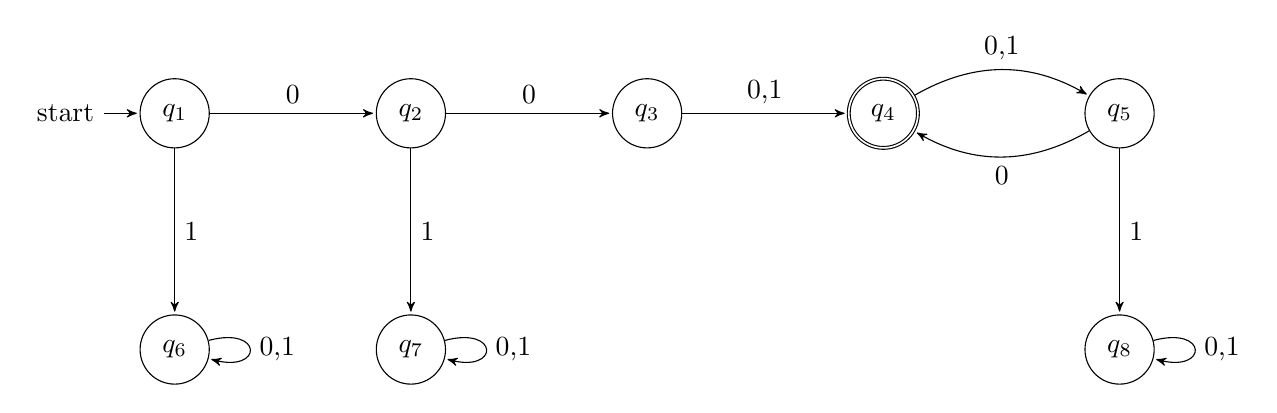
\begin{tikzpicture}[>=stealth',shorten >=1pt,auto,node distance=3cm]

\node[initial,state	]   (q1)      				{$q_1$};
 \node[state] 	  (q2) [right of=q1]  	{$q_2$};
	\node[state]   (q3) [right of=q2]      				{$q_3$};
		\node[state,accepting]   (q4) [right of=q3]      				{$q_4$};
		\node[state]   (q5) [right of=q4]      				{$q_5$};
		\node[state]   (q6) [below of=q1]      				{$q_6$};
		\node[state]   (q7) [below of=q2]      				{$q_7$};
		\node[state]   (q8) [below of=q5]      				{$q_8$};
	
	\path[->] (q1)  edge	  	node{0} 	(q2)
							
									edge  node{1} 		 	(q6)
	
					(q2) edge  node{0} 		 	(q3)
							
								edge  node{1} 		 	(q7)
														
					(q3) edge  node{0,1} 		 	(q4)
					(q4) edge[bend left]  node{0,1} 		 	(q5)
					(q5) edge[bend left]  node{0} 		 	(q4)
								edge  node{1} 		 	(q8)
					(q6) edge[loop right]  node{0,1} 		 	(q6)
					(q7) edge[loop right]  node{0,1} 		 	(q7)
						(q8) edge[loop right]  node{0,1} 		 	(q8);
						
	\end{tikzpicture}
	
\noindent\textbf{k.}
\\
\\
\\
	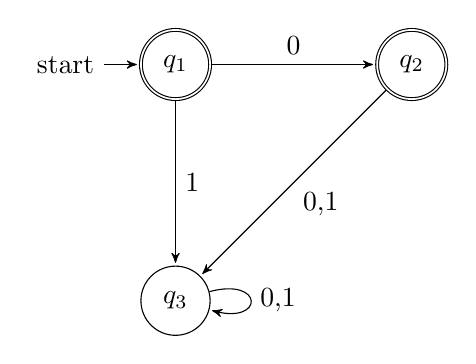
\begin{tikzpicture}[>=stealth',shorten >=1pt,auto,node distance=3cm]

\node[initial,state,accepting	]   (q1)      				{$q_1$};
 \node[state,accepting] 	  (q2) [right of=q1]  	{$q_2$};
	\node[state]   (q3) [below of=q1]      				{$q_3$};
	

	
	\path[->] (q1)  edge	  	node{0} 	(q2)
							
									edge  node{1} 		 	(q3)
	
					(q2) edge  node{0,1} 		 	(q3)
							
						(q3) edge[loop right]  node{0,1} 		 	(q3);	
				
						
	\end{tikzpicture}
	
\noindent\textbf{l.}	
\\
\\
\\
	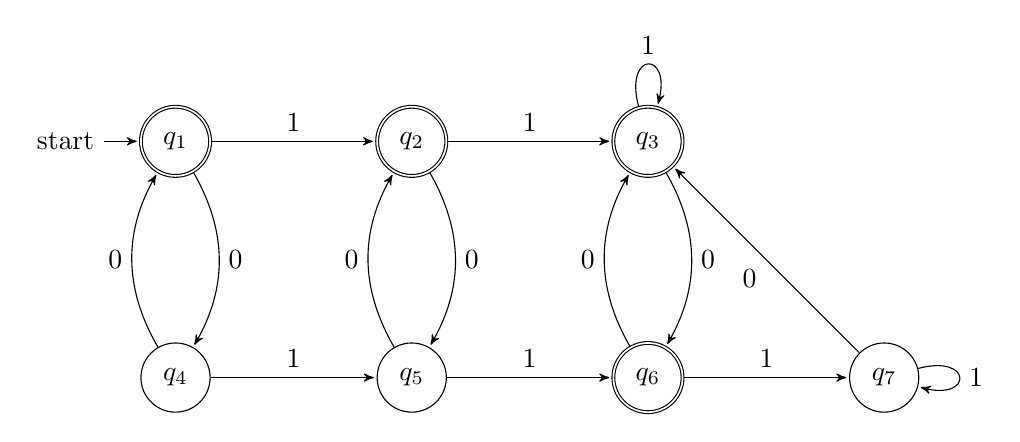
\begin{tikzpicture}[>=stealth',shorten >=1pt,auto,node distance=3cm]

\node[initial,state,accepting	]   (q1)      				{$q_1$};
 \node[state,accepting] 	  (q2) [right of=q1]  	{$q_2$};
 \node[state,accepting] 	  (q3) [right of=q2]  	{$q_3$};

	\node[state]   (q4) [below of=q1]      				{$q_4$};
	\node[state]   (q5) [below of=q2]      				{$q_5$};
\node[state,accepting]   (q6) [below of=q3]      				{$q_6$};
\node[state]   (q7) [right of=q6]      				{$q_7$};
	
	\path[->] (q1)  edge	  	node{1} 	(q2)
									
									edge[bend left]  node{0} 		 	(q4)
	
					(q2) edge  node{1} 		 	(q3)
								edge[bend left]  node{0} 		 	(q5)
							
						(q3) edge[loop above]  node{1} 		 	(q3)
									 edge[bend left]  node{0} 		 	(q6)
							
						(q4) edge  node{1} 		 	(q5)
									 edge[bend left]  node{0} 		 	(q1)
						(q5) edge  node{1} 		 	(q6)
									 edge[bend left]  node{0} 		 	(q2)			
							(q6) edge  node{1} 		 	(q7)
									 edge[bend left]  node{0} 		 	(q3)	
							(q7) edge[loop right]  node{1} 		 	(q7)
									 edge node{0} 		 	(q3);			
						
	\end{tikzpicture}
\\
\noindent\textbf{m.}
\\
	\\
	\\
	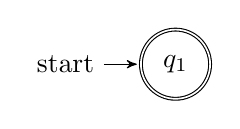
\begin{tikzpicture}[>=stealth',shorten >=1pt,auto,node distance=3cm]

\node[initial,state,accepting	]   (q1)      				{$q_1$};
 
				
				
						
	\end{tikzpicture}
	
	\noindent\textbf{n.}
	\\
	\\
	\\
	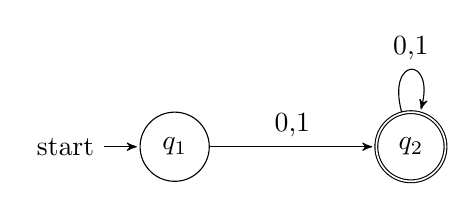
\begin{tikzpicture}[>=stealth',shorten >=1pt,auto,node distance=3cm]

\node[initial,state	]   (q1)      				{$q_1$};
 \node[state,accepting] 	  (q2) [right of=q1]  	{$q_2$};

	

	
	\path[->] (q1)  edge	  	node{0,1} 	(q2)
	
					(q2) edge[loop above]  node{0,1} 		 	(q2);
				
				
						
	\end{tikzpicture}
	
	\noindent$\textbf{1.7}$
	\\
	\\
	\\
	\noindent\textbf{b.}
	\\
	\\
	\\
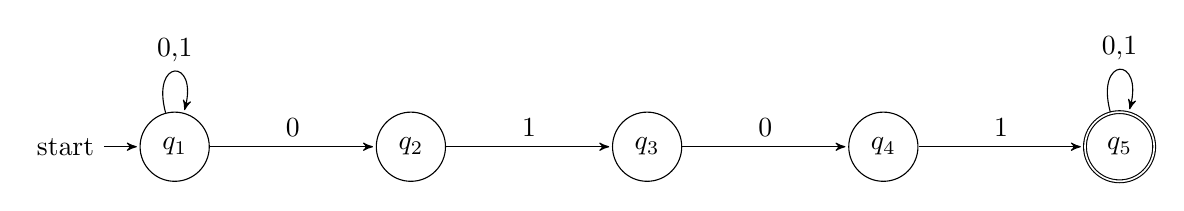
\begin{tikzpicture}[>=stealth',shorten >=1pt,auto,node distance=3cm]

\node[initial,state	]   (q1)      				{$q_1$};
 \node[state] 	  (q2) [right of=q1]  	{$q_2$};
 \node[state] 	  (q3) [right of=q2]  	{$q_3$};
	\node[state] 	  (q4) [right of=q3]  	{$q_4$};
	\node[state,accepting] 	  (q5) [right of=q4]  	{$q_5$};

	
	\path[->] (q1)  edge[loop above]	  	node{0,1} 	(q1)
								edge	  	node{0} 	(q2)
						(q2)  edge	  	node{1} 	(q3)
							(q3)  edge	  	node{0} 	(q4)
						(q4)  edge	  	node{1} 	(q5)
						(q5)  edge[loop above]	  	node{0,1} 	(q5);
	\end{tikzpicture}

\noindent\textbf{c.}
\\
\\
\\
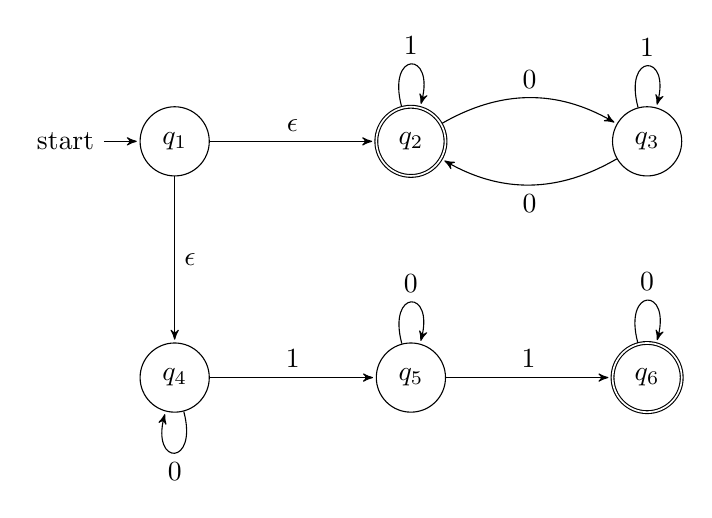
\begin{tikzpicture}[>=stealth',shorten >=1pt,auto,node distance=3cm]

\node[initial,state	]   (q1)      				{$q_1$};
 \node[state,accepting] 	  (q2) [right of=q1]  	{$q_2$};
 \node[state] 	  (q3) [right of=q2]  	{$q_3$};
	\node[state] 	  (q4) [below of=q1]  	{$q_4$};
	\node[state] 	  (q5) [right of=q4]  	{$q_5$};
		\node[state,accepting] 	  (q6) [right of=q5]  	{$q_6$};
	
	\path[->] (q1)  edge	  	node{$\epsilon$} 	(q2)
								edge	  	node{$\epsilon$} 	(q4)
						(q2)  edge[loop above]	  	node{1} 	(q2)
									edge[bend left]	  	node{0} 	(q3)
							(q3)  edge[loop above]	  	node{1} 	(q3)
										edge[bend left]	  	node{0} 	(q2)
						(q4)  edge	  	node{1} 	(q5)
									edge[loop below]	  	node{0} 	(q4)
									
						(q5)  edge[loop above]	  	node{0} 	(q5)
									edge	  	node{1} 	(q6)
						(q6)  edge[loop above]	  	node{0} 	(q6);
	\end{tikzpicture}
	
\noindent\textbf{d.}
\\
\\
\\
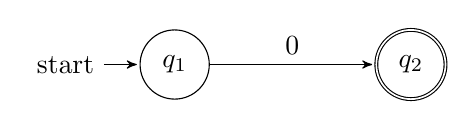
\begin{tikzpicture}[>=stealth',shorten >=1pt,auto,node distance=3cm]

\node[initial,state	]   (q1)      				{$q_1$};
 \node[state,accepting] 	  (q2) [right of=q1]  	{$q_2$};

	

	
	\path[->] (q1)  edge	  	node{0} 	(q2);
	
				
				
				
						
	\end{tikzpicture}
	
\noindent\textbf{e.}
\\
\\
\\

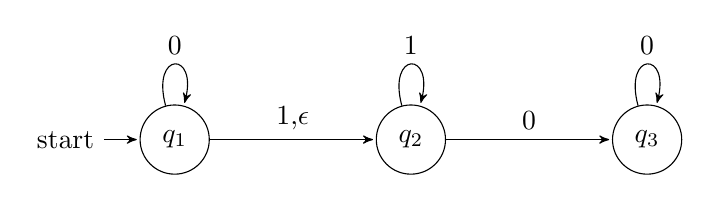
\begin{tikzpicture}[>=stealth',shorten >=1pt,auto,node distance=3cm]


\node[initial,state	]   (q1)      				{$q_1$};
 \node[state] 	  (q2) [right of=q1]  	{$q_2$};
 \node[state] 	  (q3) [right of=q2]  	{$q_3$};
	

	
	\path[->] (q1)  edge[loop above]	  	node{0} 	(q1)
									edge	  	node{1,$\epsilon$} 	(q2)
							
						(q2)  edge[loop above]	  	node{1} 	(q2)
									 edge  	node{0} 	(q3)
						(q3)  edge[loop above]	  	node{0} 	(q3);
	\end{tikzpicture}				

\noindent\textbf{g.}
\\
	\\
	\\
	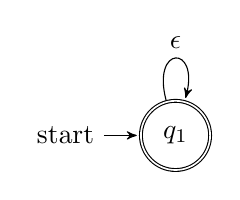
\begin{tikzpicture}[>=stealth',shorten >=1pt,auto,node distance=3cm]


\node[initial,state,accepting	]   (q1)      				{$q_1$};

	

	
	\path[->] (q1)  edge[loop above]	  	node{$\epsilon$} 	(q1);
									
	\end{tikzpicture}
	
\noindent\textbf{h.}
\\
	\\
	\\
	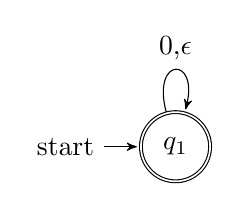
\begin{tikzpicture}[>=stealth',shorten >=1pt,auto,node distance=3cm]


\node[initial,state,accepting	]   (q1)      				{$q_1$};

	\path[->] (q1)  edge[loop above]	  	node{0,$\epsilon$} 	(q1);
									
	\end{tikzpicture}	

\noindent$\textbf{1.8}$
\\
\\
\\
\noindent\textbf{a.}
\\
\\
\\
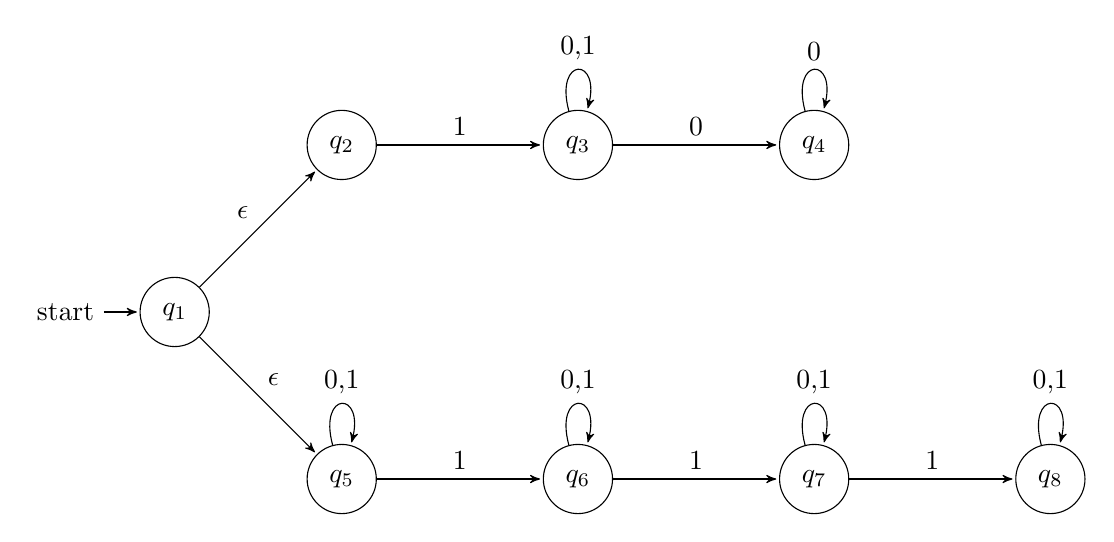
\begin{tikzpicture}[>=stealth',shorten >=1pt,auto,node distance=3cm]


\node[initial,state]   (q1)      				{$q_1$};
\node[state]   (q2)[above right of=q1]      				{$q_2$};
\node[state]   (q3)[right of=q2]      				{$q_3$};
\node[state]   (q4)[right of=q3]      				{$q_4$};
\node[state]   (q5)[below right of=q1]      				{$q_5$};
\node[state]   (q6)[ right of=q5]      				{$q_6$};
\node[state]   (q7)[ right of=q6]      				{$q_7$};
\node[state]   (q8)[ right of=q7]      				{$q_8$};

	\path[->] (q1)  edge	  	node{$\epsilon$} 	(q2)
									edge	  	node{$\epsilon$} 	(q5)
						(q2)  edge	  	node{1} 	(q3)
						
						(q3)  edge[loop above]	  	node{0,1} 	(q3)
								edge	  	node{0} 	(q4)
						(q4)  edge[loop above]	  	node{0} 	(q4)
						(q5)  edge[loop above]	  	node{0,1} 	(q5)
									edge	  	node{1} 	(q6)
						(q6)  edge[loop above]	  	node{0,1} 	(q6)	
									edge	  	node{1} 	(q7)	
						(q7)  edge[loop above]	  	node{0,1} 	(q7)
								 edge  	node{1} 	(q8)
						(q8)  edge[loop above]	  	node{0,1} 	(q8);
	\end{tikzpicture}

\noindent\textbf{b.}
\\
\\
\\
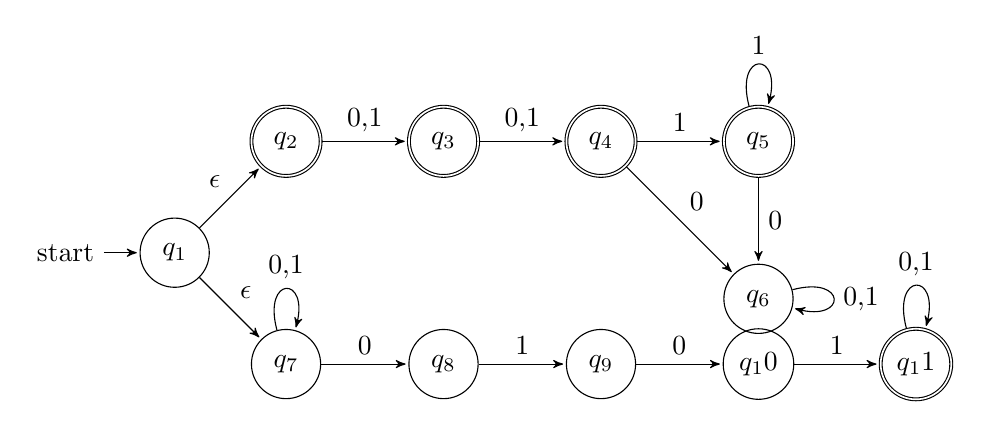
\begin{tikzpicture}[>=stealth',shorten >=1pt,auto,node distance=2cm]


\node[initial,state]   (q1)      				{$q_1$};
\node[state,accepting]   (q2)[above right of=q1]      				{$q_2$};
\node[state,accepting]  (q3)[right of=q2]      				{$q_3$};
\node[state,accepting]   (q4)[right of=q3]      				{$q_4$};
\node[state,accepting]   (q5)[right of=q4]      				{$q_5$};
\node[state]   (q6)[below of=q5]      				{$q_6$};

\node[state]   (q7)[below right of=q1]      				{$q_7$};
\node[state]   (q8)[ right of=q7]      				{$q_8$};
\node[state]   (q9)[ right of=q8]      				{$q_9$};
\node[state]   (q10)[ right of=q9]      				{$q_10$};
\node[state,accepting]   (q11)[ right of=q10]      				{$q_11$};

	\path[->] (q1)  edge	  	node{$\epsilon$} 	(q2)
									edge	  	node{$\epsilon$} 	(q7)
						(q2)  edge	  	node{0,1} 	(q3)
						
						(q3)  edge	  	node{0,1} 	(q4)
								
						(q4)  edge	  	node{0} 	(q6)
									edge	  	node{1} 	(q5)
									
						(q5)  edge[loop above]	  	node{1} 	(q5)
									edge	  	node{0} 	(q6)
						(q6)  edge[loop right]	  	node{0,1} 	(q6)	
									
									
						(q7)  edge[loop above]	  	node{0,1} 	(q7)
								 edge  	node{0} 	(q8)
						(q8)  edge	  	node{1} 	(q9)
						(q9)  edge	  	node{0} 	(q10)
						(q10)  edge	  	node{1} 	(q11)
						(q11)  edge[loop above]  	node{0,1} 	(q11);
	\end{tikzpicture}

\noindent$\textbf{1.9}$
\\
\\
\\
\noindent\textbf{a.}
\\
\\
\\
\begin{tikzpicture}[>=stealth',shorten >=1pt,auto,node distance=3cm]


\node[initial,state]   (q1)      				{$q_1$};
\node[state]   (q2)[below of=q1]      				{$q_2$};
\node[state]   (q3)[below of=q2]      				{$q_3$};
\node[state]   (q4)[below of=q3]      				{$q_4$};
\node[state]   (q5)[below  of=q4]      				{$q_5$};
\node[state]   (q6)[ below of=q5]      				{$q_6$};
\node[state]   (q7)[ right of=q6]      				{$q_7$};
\node[state]   (q8)[ right of=q3]      				{$q_8$};
\node[state,accepting]   (q9)[ right of=q8]      				{$q_9$};
\node[state]   (q10)[below of=q8]      				{$q_10$};

	\path[->] (q1)  edge	  	node{$\epsilon$} 	(q8)
									edge	  	node{0,1} 	(q2)
						(q2)  edge	  	node{0,1} 	(q3)
									edge	  	node{$\epsilon$} 	(q8)
						(q3)  edge	  	node{0,1} 	(q4)
									edge	  	node{$\epsilon$} 	(q8)
						(q4)  edge	  	node{0,1} 	(q5)
									edge	  	node{$\epsilon$} 	(q8)
						(q5)  edge	  	node{0,1} 	(q6)
									edge	  	node{$\epsilon$} 	(q8)
						(q6)  edge	  	node{0,1} 	(q7)	
						(q7)  edge[loop above]	  	node{0,1} 	(q7)
								
						(q8)  edge[bend right]	  	node{1} 	(q9)
									edge  	node{0} 	(q10)
						(q9)  edge[bend right]	  	node{0,1} 	(q8)
						(q10)  edge[loop right]	  	node{0,1} 	(q10);
	\end{tikzpicture}
	
\noindent\textbf{b.}
\\
\\
\\
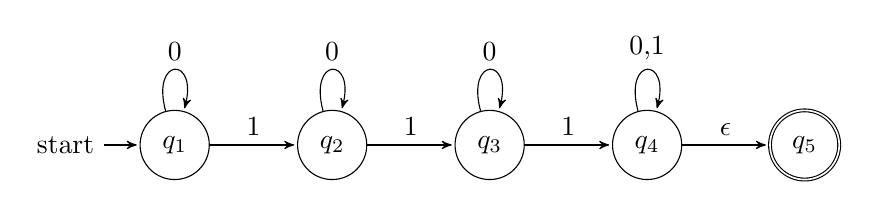
\begin{tikzpicture}[>=stealth',shorten >=1pt,auto,node distance=2cm]


\node[initial,state]   (q1)      				{$q_1$};
\node[state]   (q2)[right of=q1]      				{$q_2$};
\node[state]  (q3)[right of=q2]      				{$q_3$};
\node[state]   (q4)[right of=q3]      				{$q_4$};
\node[state,accepting]   (q5)[right of=q4]      				{$q_5$};




	\path[->] (q1)  edge[loop above]	  node{0} 	(q1)
									edge	  	node{1} 	(q2)
						(q2)  edge[loop above]	  	node{0} 	(q2)
									edge	  	node{1} 	(q3)
						(q3)  edge[loop above]	  	node{0} 	(q3)
									edge	  	node{1} 	(q4)
				
						(q4)  edge[loop above]	  	node{0,1} 	(q4)
									edge	  	node{$\epsilon$} 	(q5);
									
			
									
						
	\end{tikzpicture}
	
\noindent$\textbf{1.10}$
\\
\\
\\
\noindent\textbf{a.}
\\
\\
\\
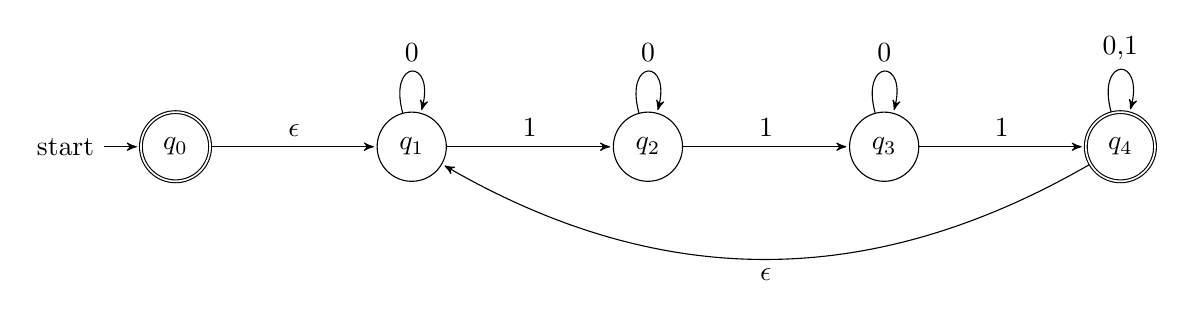
\begin{tikzpicture}[>=stealth',shorten >=1pt,auto,node distance=3cm]

\node[state,initial,accepting]   (q0)      				{$q_0$};
\node[state]   (q1)[right of=q0]      				{$q_1$};
\node[state]   (q2)[right of=q1]      				{$q_2$};
\node[state]   (q3)[right of=q2]      				{$q_3$};
\node[state,accepting]   (q4)[right of=q3]      				{$q_4$};


	\path[->] (q0)  edge	  	node{$\epsilon$} 	(q1)
									
						(q1)  edge[loop above]	  	node{0} 	(q1)
									edge	  	node{1} 	(q2)
						(q2)  edge[loop above]	 node{0} 	(q2)
									edge	  	node{1} 	(q3)
						(q3)  edge[loop above]	  	node{0} 	(q3)
									edge	  	node{1} 	(q4)
						(q4)  edge[loop above]	  	node{0,1} 	(q4)
									edge[bend left]	  	node{$\epsilon$} 	(q1);
		
	\end{tikzpicture}
	
\noindent\textbf{b.}
\\
\\
\\	
	
	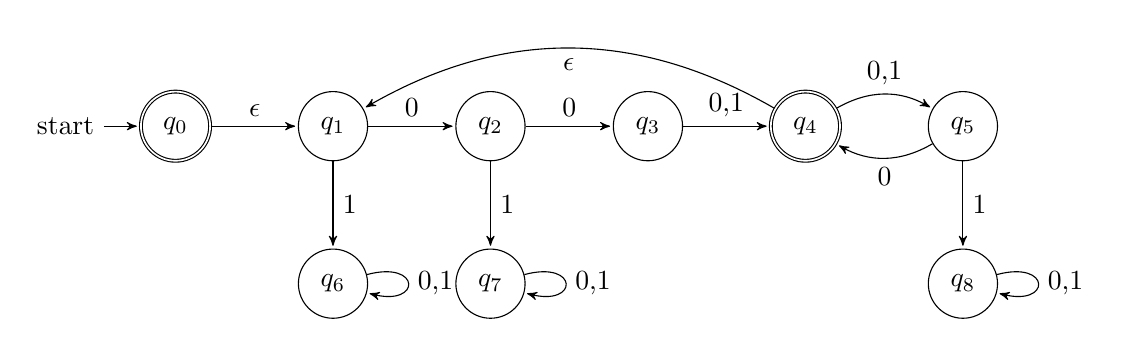
\begin{tikzpicture}[>=stealth',shorten >=1pt,auto,node distance=2cm]
\node[state,initial,accepting	]   (q0)      				{$q_0$};
\node[state	]   (q1) [right of=q0]     				{$q_1$};
 \node[state] 	  (q2) [right of=q1]  	{$q_2$};
	\node[state]   (q3) [right of=q2]      				{$q_3$};
		\node[state,accepting]   (q4) [right of=q3]      				{$q_4$};
		\node[state]   (q5) [right of=q4]      				{$q_5$};
		\node[state]   (q6) [below of=q1]      				{$q_6$};
		\node[state]   (q7) [below of=q2]      				{$q_7$};
		\node[state]   (q8) [below of=q5]      				{$q_8$};
	
	\path[->] (q0)  edge	  	node{$\epsilon$} 	(q1)
					
					(q1)  edge	  	node{0} 	(q2)
							
									edge  node{1} 		 	(q6)
	
					(q2) edge  node{0} 		 	(q3)
							
								edge  node{1} 		 	(q7)
														
					(q3) edge  node{0,1} 		 	(q4)
					(q4) edge[bend left]  node{0,1} 		 	(q5)
								edge[bend right]  node{$\epsilon$} 		 	(q1)
					(q5) edge[bend left]  node{0} 		 	(q4)
								edge  node{1} 		 	(q8)
					(q6) edge[loop right]  node{0,1} 		 	(q6)
					(q7) edge[loop right]  node{0,1} 		 	(q7)
						(q8) edge[loop right]  node{0,1} 		 	(q8);
						
	\end{tikzpicture}


\noindent\textbf{c.}
\\
\\
\\
	
	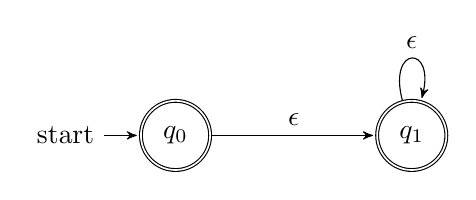
\begin{tikzpicture}[>=stealth',shorten >=1pt,auto,node distance=3cm]

\node[state,initial,accepting	]   (q0)      				{$q_0$};

\node[state,accepting	]   (q1)[right of=q0]      				{$q_1$};
 
	\path[->] (q0)  edge	  	node{$\epsilon$} 	(q1)		
				 (q1)  edge[loop above]	  	node{$\epsilon$} 	(q1);
						
	\end{tikzpicture}
	
\noindent$\textbf{1.12}$
\\
\\
\\
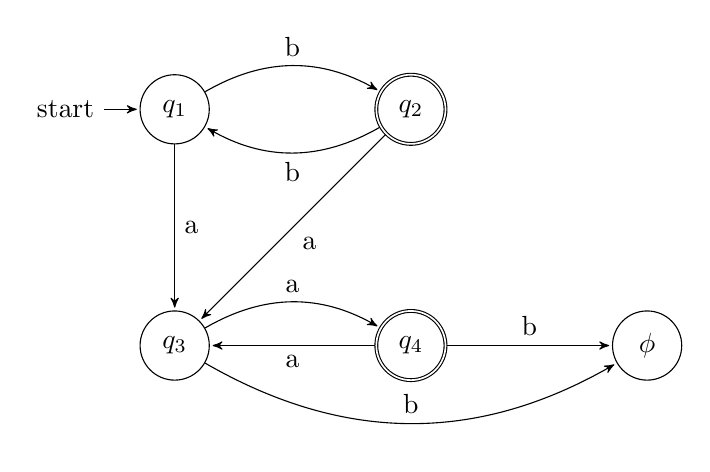
\begin{tikzpicture}[>=stealth',shorten >=1pt,auto,node distance=3cm]

\node[state,initial]   (q1)      				{$q_1$};
\node[state,accepting]   (q2)[right of=q1]      				{$q_2$};
\node[state]   (q3)[below of=q1]      				{$q_3$};
\node[state,accepting]   (q4)[right of=q3]      				{$q_4$};
\node[state	]   (phi)[right of=q4]      				{$\phi$};
 
	\path[->] (q1)  edge[bend left]	  	node{b} 	(q2)
									edge	  	node{a} 	(q3)
							(q2)  edge[bend left]	  	node{b} 	(q1)
									edge	  	node{a} 	(q3)
						(q3)  edge[bend left]	  	node{a} 	(q4)
									edge[bend right]	  	node{b} 	(phi)
				 (q4)  edge	  	node{a} 	(q3)
								edge	  	node{b} 	(phi);
	\end{tikzpicture}

regular expression:\, $b(bb)^*(aa)^*$
\\
\\
\\
\noindent$\textbf{1.13}$
\\
\\
\\
step 1) 4-state NFA recognizing a pair of 1 with an odd number of symbols in between
\\
\\
\\
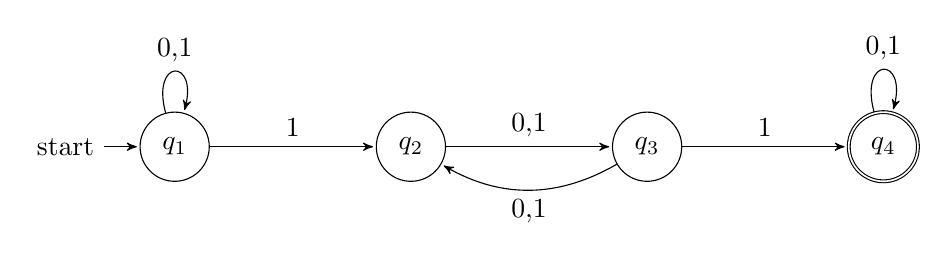
\begin{tikzpicture}[>=stealth',shorten >=1pt,auto,node distance=3cm]

\node[state,initial]   (q1)      				{$q_1$};
\node[state]   (q2)[right of=q1]      				{$q_2$};
\node[state]   (q3)[right of=q2]      				{$q_3$};
\node[state,accepting]   (q4)[right of=q3]      				{$q_4$};

 
	\path[->] (q1)  edge[loop above]	  	node{0,1} 	(q1)
									edge	  	node{1} 	(q2)
							(q2)  edge  	node{0,1} 	(q3)
									
						(q3)  edge	  	node{1} 	(q4)
									edge[bend left]	  	node{0,1} 	(q2)
				 (q4)  edge[loop above]	  	node{0,1} 	(q4);
							
\end{tikzpicture}
	
step 2) convert the NFA to the corresponding DFA
\\
\\
\\
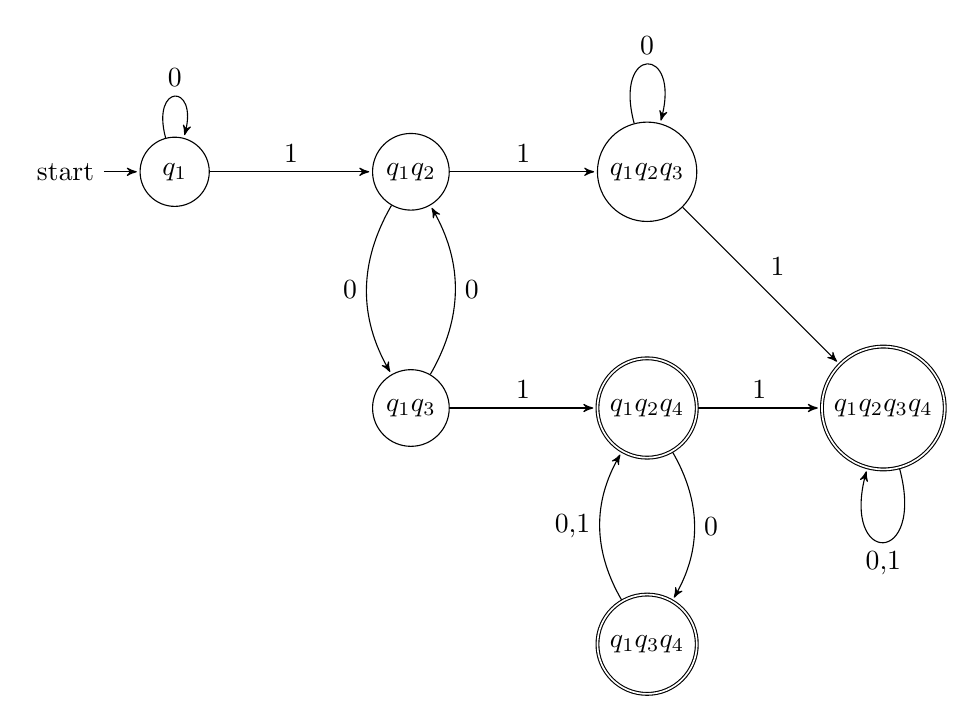
\begin{tikzpicture}[>=stealth',shorten >=1pt,auto,node distance=3cm]

\node[state,initial]   (q1)      				{$q_1$};
\node[state]   (q12)[right of=q1]      				{$q_1q_2$};
\node[state]   (q123)[right of=q12]      				{$q_1q_2q_3$};
\node[state]   (q13)[below of=q12]      				{$q_1q_3$};
\node[state,accepting]   (q124)[right of=q13]      				{$q_1q_2q_4$};
\node[state,accepting]   (q1234)[right of=q124]      				{$q_1q_2q_3q_4$};
\node[state,accepting]   (q134)[below of=q124]      				{$q_1q_3q_4$};
 
	\path[->] (q1)  edge[loop above]	  	node{0} 	(q1)
									edge	  	node{1} 	(q12)
							(q12)  edge  	node{1} 	(q123)
											edge[bend right,left]  node{0}  (q13)
											
							(q123)  edge[loop above]  	node{0} 	(q123)
											edge  node{1}  (q1234)
						(q13)  edge[bend right,right]	  	node{0} 	(q12)
										edge	  	node{1} 	(q124)
						(q124)  edge	  	node{1} 	(q1234)
										edge[bend left,right]	  	node{0} 	(q134)
						(q1234)  edge[loop below]	  	node{0,1} 	(q1234)
						(q134)  edge[bend left]	  	node{0,1} 	(q124);
									
										
	\end{tikzpicture}



step 3) complement and minimize the states of the DFA above
\\
\\
\\
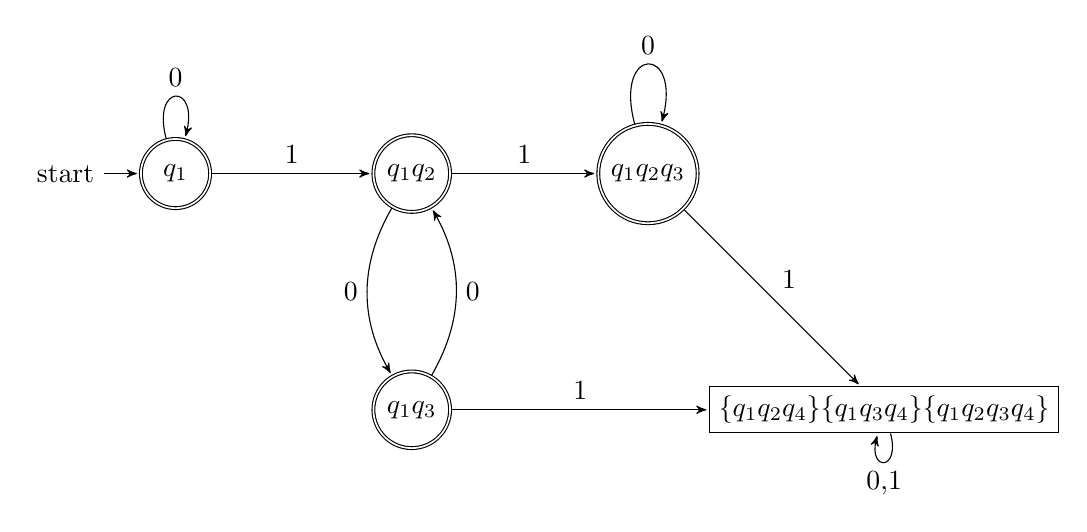
\begin{tikzpicture}[>=stealth',shorten >=1pt,auto,node distance=3cm]

\node[state,initial,accepting]   (q1)      				{$q_1$};
\node[state,accepting]   (q12)[right of=q1]      				{$q_1q_2$};
\node[state,accepting]   (q123)[right of=q12]      				{$q_1q_2q_3$};
\node[state,accepting]   (q13)[below of=q12]      				{$q_1q_3$};
\node[draw, rectangle]   (q0)[ right of=q123,below of=q123]      								{$\{q_1q_2q_4\} \\ \{q_1q_3q_4\} \\ \{q_1q_2q_3q_4\}$};

 
	\path[->] (q1)  edge[loop above]	  	node{0} 	(q1)
									edge	  	node{1} 	(q12)
							(q12)  edge  	node{1} 	(q123)
											edge[bend right,left]  node{0}  (q13)
											
							(q123)  edge[loop above]  	node{0} 	(q123)
											edge  node{1}  (q0)
						(q13)  edge[bend right,right]	  	node{0} 	(q12)
										edge	  	node{1} 	(q0)
						(q0)  edge[loop below]	  	node{0,1} 	(q0);
						
									
										
	\end{tikzpicture}

\noindent$\textbf{1.16}$
\\
\\
\\
\noindent\textbf{a.}
\\
\\
\\
	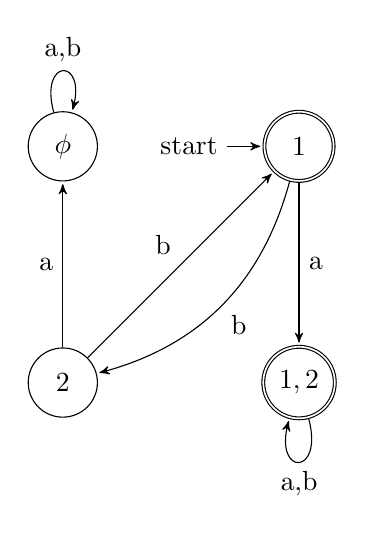
\begin{tikzpicture}[>=stealth',shorten >=1pt,auto,node distance=3cm]

\node[state,initial,accepting	]   (1)      				{${1}$};
\node[state	]   (phi)[left of=1]      				{$\phi$};
\node[state	]   (2)[below of=phi]      				{${2}$};
 \node[state,accepting	]   (12)[right of=2]      			{${1,2}$};

	\path[->] (1)  edge[bend left]	  	node{b} 	(2)
									edge		node{a} 	(12)
				 (phi)  edge[loop above]	  	node{a,b} 	(phi)
					(2)  edge	  	node{b} 	(1)
									edge		node{a} 	(phi)
						(12)  edge[loop below]	  	node{a,b} 	(12);
									
	\end{tikzpicture}
	
\noindent\textbf{b.}
\\
\\
\\
	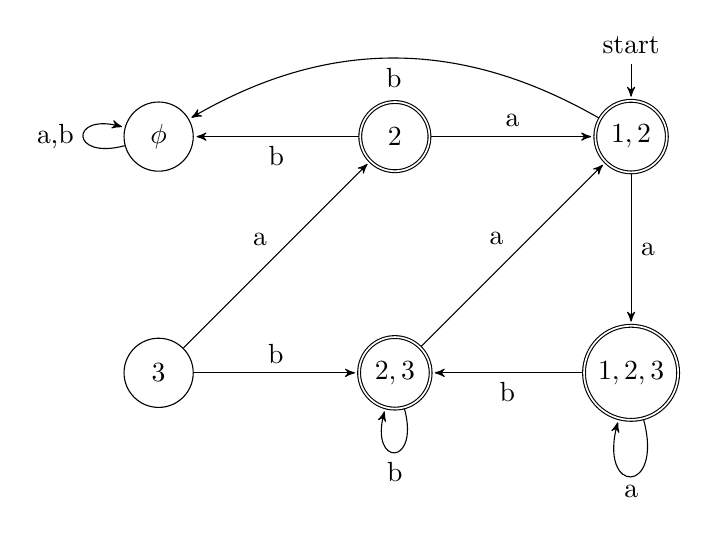
\begin{tikzpicture}[>=stealth',shorten >=1pt,auto,node distance=3cm]

\node[state	]   (phi)      				{$\phi$};
\node[state,accepting	]   (2)[right of=phi]      				{$2$};
\node[state,accepting,initial,initial where=above	]   (12)[right of=2]      				{$1,2$};
 \node[state	]   (3)[below of=phi]      			{$3$};
 \node[state,accepting	]   (23)[right of=3]      			{$2,3$};
\node[state,accepting	]   (123)[right of=23]      			{$1,2,3$};

	\path[->] (phi)  edge[loop left]	  	node{a,b} 	(phi)
								
				 (2)  edge	  	node{b} 	(phi)
							edge	  	node{a} 	(12)
							
					(12)  edge	  	node{a} 	(123)
								edge[bend right]	  	node{b} 	(phi)
			
						(3)  edge	  	node{a} 	(2)
								edge	  	node{b} 	(23)
						(23)  edge	  	node{a} 	(12)	
									edge[loop below]	  	node{b} 	(23)
							(123)  edge	  	node{b} 	(23)	
										  edge[loop below]	  	node{a} 	(123);
	\end{tikzpicture}
	
	\noindent$\textbf{1.17}$
	\\
	\\
	\\
	\noindent\textbf{a.}
	\\
	\\
	\\
	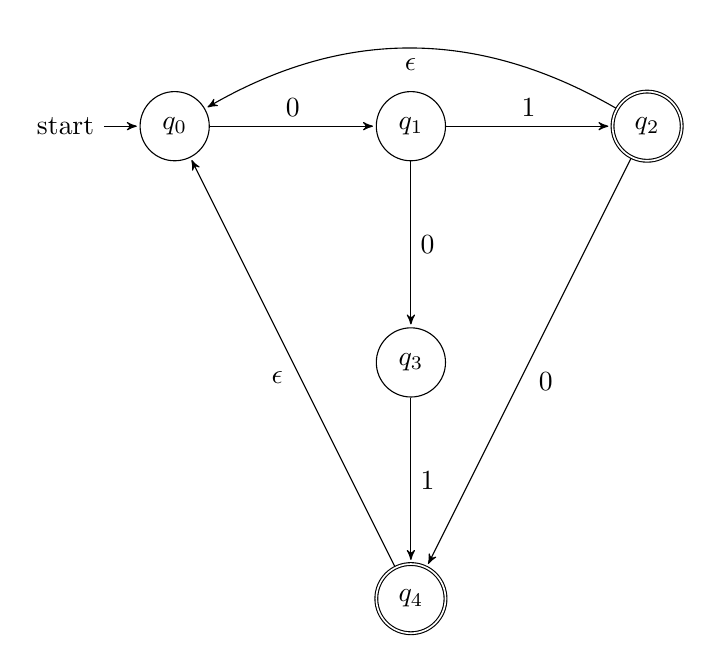
\begin{tikzpicture}[>=stealth',shorten >=1pt,auto,node distance=3cm]

\node[state,initial]   (q0)      				{$q_0$};
\node[state]   (q1)[right of=q0]      				{$q_1$};
\node[state,accepting]   (q2)[right of=q1]      				{$q_2$};
\node[state]   (q3)[below of=q1]      				{$q_3$};
\node[state,accepting]   (q4)[below of=q3]      				{$q_4$};


	\path[->] (q0)  edge	  	node{0} 	(q1)
									
						(q1)  edge	  	node{1} 	(q2)
									edge	  	node{0} 	(q3)
						(q2)  edge[bend right]	 node{$\epsilon$} 	(q0)
									edge	  	node{0} 	(q4)
						(q3)  edge	  	node{1} 	(q4)
								
						(q4)  edge	  	node{$\epsilon$} 	(q0);
		
									
	\end{tikzpicture}

	
\noindent\textbf{b.}
\\
\\
\\
	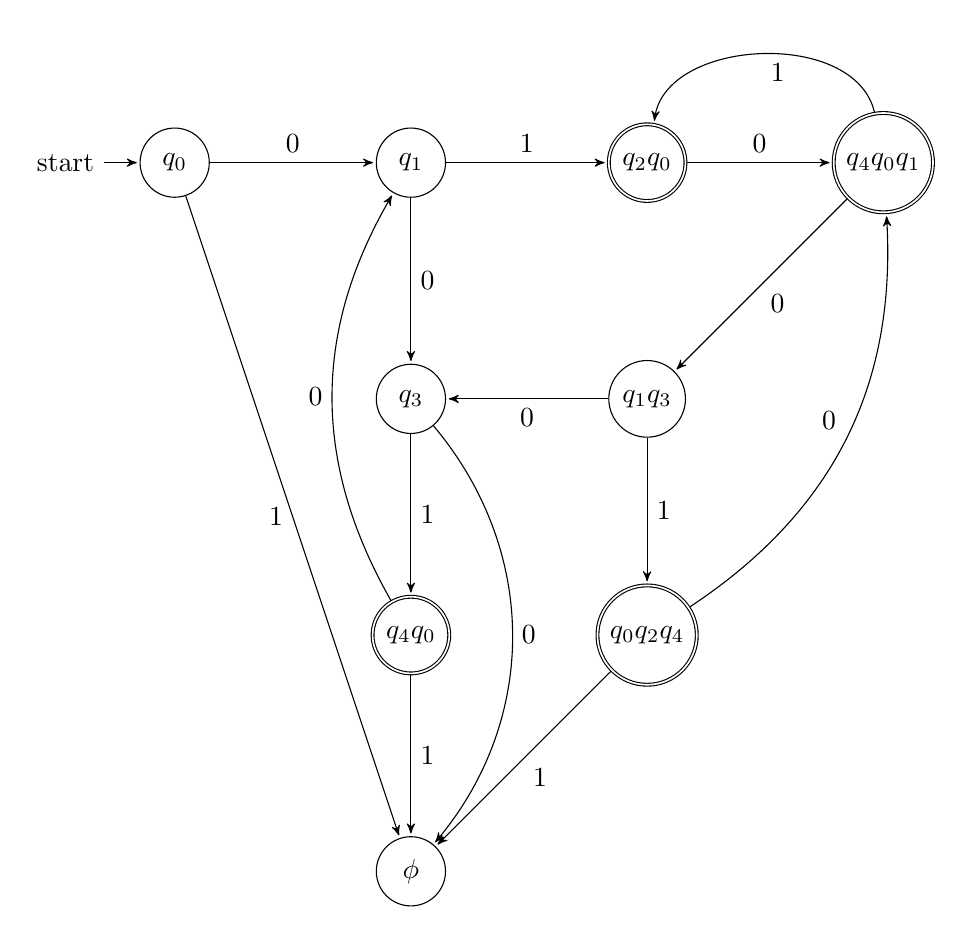
\begin{tikzpicture}[>=stealth',shorten >=1pt,auto,node distance=3cm]

\node[state,initial]   (q0)      				{$q_0$};
\node[state]   (q1)[right of=q0]      				{$q_1$};
\node[state,accepting]   (q20)[right of=q1]      				{$q_2q_0$};
\node[state,accepting]   (q401)[right of=q20]      				{$q_4q_0q_1$};
\node[state]   (q3)[below of=q1]      				{$q_3$};
\node[state]   (q13)[right of=q3]      				{$q_1q_3$};
\node[state,accepting]   (q40)[below of=q3]      				{$q_4q_0$};
\node[state,accepting]   (q024)[right of=q40]      				{$q_0q_2q_4$};
\node[state]   (phi)[below of=q40]      				{$\phi$};



	\path[->] (q0)  edge	  	node{0} 	(q1)
									edge[left]	  	node{1} 	(phi)
						(q1)  edge	  	node{1} 	(q20)
									edge	  	node{0} 	(q3)
						
						(q20)  edge	  	node{0} 	(q401)
										
						(q401)  edge[bend right=80]	  	node{1} 	(q20)
									edge	  	node{0} 	(q13)
						(q3)  edge	  	node{1} 	(q40)
									edge[bend left=40]	  	node{0} 	(phi)
						(q13)  edge	  	node{0} 	(q3)
									edge	  	node{1} 	(q024)
									
						(q40)  edge[bend left]	  	node{0} 	(q1)
										edge  	node{1} 	(phi)
						(q024)  edge[bend right]	  	node{0} 	(q401)
										edge  	node{1} 	(phi);
		
									
	\end{tikzpicture}

	\noindent$\textbf{1.18}$
	\\
\\
\\
\noindent\textbf{a.}$1\sum^*0$
\\
\noindent\textbf{b.} $\sum^*1\sum^*1\sum^*1\sum^*$
\\
\noindent\textbf{c.}$\sum^*0101\sum^*$
\\
\noindent\textbf{d.} $\sum\sum0\sum^*$
\\
\noindent\textbf{e.} $(0\cup1\sum)(\sum\sum)^*$
\\
\noindent\textbf{f.} $0^*(10^+)^*1^*$
\\
\noindent\textbf{g.}$\sum\sum\sum\sum\sum$
\\
\noindent\textbf{h.} $\sum^*\sum\sum\sum\sum\sum^*\cup\sum\cup0\sum\cup10\cup0\sum\sum\cup10\sum\cup110$
\\
\noindent\textbf{i.} $(1\sum)^*$
\\
\noindent\textbf{j.} $0^+\sum0^+\cup\sum0^+0^+\cup0^+0^+\sum$
\\
\noindent\textbf{k.} $\epsilon\cup0$
\\
\noindent\textbf{l.} $(1^*01^*01^*)^*\cup0^*10^*10^*$
\\
\noindent\textbf{m.} $\phi $
\\
\noindent\textbf{n.} $\sum^*\sum^+$
\\
\\
\\

	\noindent$\textbf{1.19}$
	\\
	\\
	\\
	\noindent\textbf{a.} 
	\\
	\\
	\\
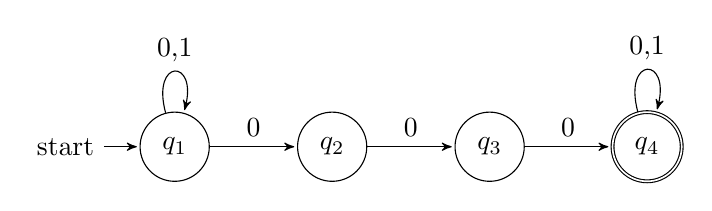
\begin{tikzpicture}[>=stealth',shorten >=1pt,auto,node distance=2cm]


\node[initial,state]   (q1)      				{$q_1$};
\node[state]   (q2)[right of=q1]      				{$q_2$};
\node[state]  (q3)[right of=q2]      				{$q_3$};
\node[state,accepting]   (q4)[right of=q3]      				{$q_4$};





	\path[->] (q1)  edge[loop above]	  node{0,1} 	(q1)
									edge	  	node{0} 	(q2)
						(q2)  edge	  	node{0} 	(q3)
							
						(q3)  edge	  	node{0} 	(q4)
								
				
						(q4)  edge[loop above]	  	node{0,1} 	(q4);
								

						
	\end{tikzpicture}

\noindent\textbf{b.}
\\
\\
\\
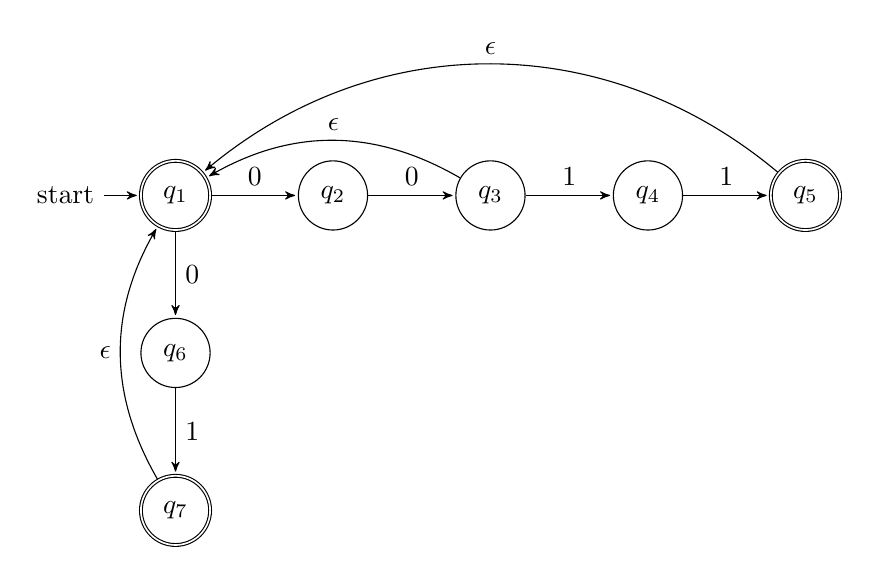
\begin{tikzpicture}[>=stealth',shorten >=1pt,auto,node distance=2cm]


\node[initial,state,accepting]   (q1)      				{$q_1$};
\node[state]   (q2)[right of=q1]      				{$q_2$};
\node[state]  (q3)[right of=q2]      				{$q_3$};
\node[state]   (q4)[right of=q3]      				{$q_4$};
\node[state,accepting]   (q5)[right of=q4]      				{$q_5$};
\node[state]   (q6)[below of=q1]      				{$q_6$};
\node[state,accepting]   (q7)[below of=q6]      				{$q_7$};
	\path[->] (q1)  edge	  node{0} 	(q2)
									edge	  	node{0} 	(q6)
						(q2)  edge	  	node{0} 	(q3)
							
						(q3)  edge	  	node{1} 	(q4)
								edge[bend right,above]	  	node{$\epsilon$} 	(q1)
				
						(q4)  edge	  	node{1} 	(q5)
							(q5)  edge[bend right=40,above]	  	node{$\epsilon$} 	(q1)
							(q6)  edge	  	node{1} 	(q7)	
						(q7)  edge[bend left]	  	node{$\epsilon$} 	(q1);
						
	\end{tikzpicture}
	
\noindent\textbf{c.}
\\
\\
\\
\\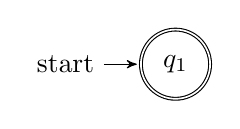
\begin{tikzpicture}[>=stealth',shorten >=1pt,auto,node distance=2cm]


\node[initial,state,accepting]   (q1)      				{$q_1$};
			
	\end{tikzpicture}
	
\noindent$\textbf{1.20}$
\\
\\	
\\
\noindent\textbf{a.}\,\underline{members}: ab, aab \qquad \underline{not members}: ba,baa\\
\noindent\textbf{b.}\,\underline{members}: abab,ab\qquad \underline{not members}: aa,a\\
\noindent\textbf{c.}\,\underline{members}: a,b\qquad \underline{not members}: ab,ba\\
\noindent\textbf{d.}\,\underline{members}: aaa,aaaaaa\qquad \underline{not members}: b,ba\\
\noindent\textbf{e.}\,\underline{members}: aba,aaba\qquad \underline{not members}: ba,b\\
\noindent\textbf{f.}\,\underline{members}: aba,bab\qquad \underline{not members}: a,b\\
\noindent\textbf{g.}\,\underline{members}: ab,b\qquad \underline{not members}: aa,a\\
\noindent\textbf{h.}\,\underline{members}: a,ba\qquad \underline{not members}: b,$\epsilon$
\\
\\
\\
\noindent$\textbf{1.21}$
\\
\\
\\
\noindent\textbf{a.}\,$a^*ba^*(ba^*ba^*)^*$
\\

\noindent\textbf{b.}\,$\sum a^*b(ba^*b)^*(a\sum a^*b(ba^*b)^*)^*$
\\
\\
\\
\noindent$\textbf{1.22}$
\\
\\
\\
\noindent\textbf{a.}
\\
\\
\\
\begin{tikzpicture}[>=stealth',shorten >=1pt,auto,node distance=2cm]


\node[initial,state]   (q1)      				{$q_1$};
\node[state]   (q2)[right of=q1]      				{$q_2$};
\node[state]  (q3)[right of=q2]      				{$q_3$};
\node[state]   (q4)[right of=q3]      				{$q_4$};
\node[state,accepting]   (q5)[right of=q4]      				{$q_5$};


	\path[->] (q1)  edge	  node{/} 	(q2)
									
						(q2)  edge	  	node{\#} 	(q3)
							
						(q3)  edge[loop above]	  	node{a,b,/} 	(q3)
									edge  	node{\#} 	(q4)

						(q4)  edge[loop above]	  	node{\#} 	(q4)
									edge[bend left]				node{a,b}  (q3)
									edge				node{/}  (q5);
								
						
	\end{tikzpicture}
	
	\noindent\textbf{b.}
\\
\\
\\
/\#(a$\cup$b$\cup$/)$^*$\#((a$\cup$b)(a$\cup$b$\cup$/)$^*$\#)$^*$\#$^*$/ \\ \\



\noindent$\textbf{1.28}$
\\
\\
\\
\noindent\textbf{a.}
\\
\\
\\
\begin{tikzpicture}[>=stealth',shorten >=1pt,auto,node distance=2cm]


\node[initial,state]   (q1)      				{$q_1$};
\node[state,accepting]   (q2)[right of=q1]      				{$q_2$};
\node[state]  (q3)[right of=q2]      				{$q_3$};
\node[state]   (q4)[right of=q3]      				{$q_4$};
\node[state]   (q5)[right of=q4]      				{$q_5$};
\node[state,accepting]   (q6)[below of=q1]      				{$q_6$};

	\path[->] (q1)  edge	  node{a} 	(q2)
									edge	  	node{b} 	(q6)
						(q2)  edge	  	node{a} 	(q3)
							
						(q3)  edge	  	node{b} 	(q4)
						
				
						(q4)  edge	  	node{b} 	(q5)
							(q5)  edge[bend right]	  	node{$\epsilon$} 	(q2);
						
						
	\end{tikzpicture}

\noindent\textbf{b.}
\\
\\
\\
\begin{tikzpicture}[>=stealth',shorten >=1pt,auto,node distance=2cm]


\node[initial,state]   (q1)      				{$q_1$};
\node[state,accepting]   (q2)[right of=q1]      				{$q_2$};
\node[state]  (q3)[below of=q1]      				{$q_3$};
\node[state]   (q4)[right of=q3]      				{$q_4$};
\node[state,accepting]   (q5)[right of=q4]      				{$q_5$};


	\path[->] (q1)  edge	  node{a} 	(q2)
									edge	  	node{$\epsilon$} 	(q3)
						(q2)  edge[loop above]	  	node{a} 	(q2)
							
						(q3)  edge	  	node{a} 	(q4)
						
				
						(q4)  edge	  	node{b} 	(q5)
							(q5)  edge[bend left]	  	node{$\epsilon$} 	(q3);
						
						
	\end{tikzpicture}
	
\noindent\textbf{c.}
\\
\\
\\
\begin{tikzpicture}[>=stealth',shorten >=1pt,auto,node distance=2cm]


\node[initial,state]   (q1)      				{$q_1$};
\node[state]   (q2)[right of=q1]      				{$q_2$};
\node[state]  (q3)[below of=q1]      				{$q_3$};
\node[state]   (q4)[right of=q2]      				{$q_4$};
\node[state,accepting]   (q5)[right of=q4]      				{$q_5$};


	\path[->] (q1)  edge	  node{a} 	(q2)
									edge	  	node{b} 	(q3)
						(q2)  edge	  	node{a} 	(q4)
							
						(q3)  edge	  	node{$\epsilon$} 	(q2)
									edge[loop below]	  	node{b} 	(q3)
				
						(q4)  edge[loop above]	  	node{a} 	(q4)
							  edge  	node{b} 	(q5)
							(q5)  edge[loop above]	  	node{b} 	(q5);
						
	\end{tikzpicture}
	

\noindent$\textbf{1.29}$
\\
\\
\\


\subsection*{a)}

 Assume that $A_1$ = \{$0^n$$1^n$$2^n$$\mid$n $\geq$ 0\} is regular. Let p be the pumping length
given by the pumping lemma. Choose s to be the string $0^p$$1^p$$2^p$. Because s is a
member of $A_1$ and s is longer than p, the pumping lemma guarantees that s can
be split into three pieces, s = xyz, where for any i $\geq$ 0 the string x$y^i$z is in $A_1$.
Consider two possibilities:
1. The string y consists only of 0s, only of 1s, or only of 2s. In these cases, the
string xyyz will not have equal numbers of 0s, 1s, and 2s. Hence xyyz is not
a member of $A_1$, a contradiction.
2. The string y consists of more than one kind of symbol. In this case, xyyz
will have the 0s, 1s, or 2s out of order. Hence xyyz is not a member of $A_1$,
a contradiction.
Either way we arrive at a contradiction. Therefore, $A_1$ is not regular.

\subsection*{b)}

Suppose that $A_2$ is a regular language. Let p be the “pumping length”
of the Pumping Lemma. Consider the string s = $a^p$b$a^p$b$a^p$b. Note that 
s $\in$ $A_2$,since s = ($a^p$b)$^3$, and $\mid$ s$\mid$ = 3($p + 1$) $\geq$ p, 
so the Pumping Lemma will hold. Thus, we can split the string s into 3 parts $s = xyz$
 \\satisfying the conditions:1)x$y^i$z$\in$$A_2$ for each i $\geq$ 0;2)$\mid$y$\mid$$>$0;
3)$\mid$xy$\mid$ $\leq$p. Since the first p symbols of s are all a, the third condition
implies that x and y consist only of a. So z will be the rest of the first set of a,
followed by b$a^p$b$a^p$b. The second condition states that $\mid$y$\mid$ $>$ 0, so y has at
 least one a. More precisely, we can then say that \\
x=$a^j$ for some j$\geq$0,\\
y=$a^k$ for some k$\geq$1,\\
z=$a^m$b$a^p$b$a^p$b for some m$\geq$0.\\
Since $a^p$b$a^p$b$a^p$b=s=xyz=$a^j$$a^k$$a^m$b$a^p$b$a^p$b=$a^{j+k+m}$b$a^p$b$a^p$b,we must
have that$ j+k+m = p$. The first condition implies that x$y^2$z $\in$ $A_2$,but 
x$y^2$z=$a^j$$a^k$$a^k$$a^m$b$a^p$b$a^p$b\\
  = $a^{p+k}$b$a^p$b$a^p$b\\
since  $j + k + m = p$. Hence,x$y^2$z$\notin$ $A_2$ because k $\geq$ 1, and we get a contradiction.
Therefore, $A_2$ is a nonregular language.





\subsection*{c)}


Assume that $A_3 = \{a^{2^n}\mid n \geq 0\} $is regular. Let p be the pumping length given
by the pumping lemma. Choose s to be the string $2^p$. Because s is a member of
$A_3$ and s is longer than p, the pumping lemma guarantees that s can be split into
three pieces, s = xyz, satisfying the three conditions of the pumping lemma.
The third condition tells us that $\mid xy \mid \leq p$. Furthermore, $p < 2^p$ and so $\mid y\mid < 2^p$.
Therefore, $\mid xyyz \mid  = \mid xyz \mid+ \mid y \mid < 2^p+2^p = 2^{p+1}$. The second condition requires
$\mid y \mid > 0$ so $2^p < \mid xyyz \mid < 2^{p+1}$. The length of xyyz cannot be a power of 2. Hence
xyyz is not a member of $A_3$, a contradiction. Therefore, $A_3$ is not regular.
\\
\\
\\
\noindent$\textbf{1.31}$
\\
\\

One solution is recursively (or inductively) define a reversing operation on regular
expressions, and apply that operation on the regular expression for A. In particular, given a
regular expression R, reverse(R) is:

\begin{itemize}

\item a for some a $\in$ Σ,
\item $\epsilon$ if R = $\epsilon$ ,
\item $\phi$ if R = $\phi$ ,
\item (reverse($R_1$) $\cup$ reverse($R_2$)), if R = $R_1$ $\cup$ $R_2$,
\item	(reverse($R_2$) $\circ$ reverse($R_1$)) if R = $R_1$ $\circ$ $R_2$, or 
\item (reverse$(R_1)^*$), if R = ($R^*_1$)

\end{itemize}

Let M = (Q,$\sum$,$\delta$,s,F) be a NFA that accepts L. Create a NFA R = (Q$\cup${r},$\sum$,$\gamma$,r,\{s\}) to accept $L^R$.r is a new state not in Q.$\gamma$ reverse the transitions in $\delta$,i.e. for each (q,c)$\to$ q$\prime$ in $\delta$ there is a (q$\prime$,c)
$\to$ q in $\gamma$. Also $\gamma$ contains $\epsilon$ transitions from r to every state in F. Thus there exists a sequence of transitions from s to a state in F in M on input w iff there exists a sequence of transitions from r to s in R on input $w^R$.

\end{document}